\documentclass[12pt,letterpaper]{article}
\usepackage{amsmath}
\usepackage{gensymb}
\usepackage[inline]{enumitem}
\usepackage{graphicx}
\usepackage[margin=1in]{geometry}
\setlength{\parindent}{0pt}
\title{Physics Club Practice Test 4}
\usepackage[export]{adjustbox}
\usepackage[none]{hyphenat}
\usepackage{titlesec}
\titlespacing{\section}{0pt}{4.0ex plus .2ex}{-3.3ex}
\titlespacing{\paragraph}{0pt}{0pt}{1em}
% \setenumerate[2]{label={\alph*.}}
\usepackage{fancyhdr}
\fancypagestyle{firstpage}
{
	\renewcommand{\headrulewidth}{0pt}
	\renewcommand{\footrulewidth}{0.4pt}
	\lfoot{Physics Club}
	\cfoot{$F=ma$ Practice Test 4}
	\rfoot{\thepage}
}
\thispagestyle{firstpage}
\pagestyle{fancy}
\fancyhf{}
\renewcommand{\headrulewidth}{0pt}
\renewcommand{\footrulewidth}{0.4pt}
\lfoot{Physics Club}
\cfoot{$F=ma$ Practice Test 4}
\rfoot{\thepage}
\setenumerate{leftmargin=*}
\begin{document}
\section*{Physics Club: $F=ma$ Practice Test 4}\hfill Version 1.0
\vspace{-2.5pt}
\begin{center}
\textsc{25 Questions -- 75 Minutes}
\end{center}
\vspace{-5pt}
Assume the acceleration due to gravity near the surface of the Earth $g = 10$ m/s$^2$.
\smallskip

Correct answers will be awarded one point; incorrect answers will result in a deduction of 1/4 point. There is no penalty for leaving an answer blank.
\smallskip

You may use a scientific calculator. Its memory must be cleared of data and programs.
\vspace{-7.5pt}

\hrulefill
\vspace{-7.5pt}
\begin{enumerate}
\item
A tennis ball is released from rest and allowed to fall onto a hard surface. The graph below shows how the velocity of the bouncing ball varies with time from the instant of release. At which point indicated does the ball reach its maximum height after the first bounce?

\begin{tabular}{l r}

\begin{minipage}{0.4\textwidth}
\begin{enumerate}
\item A
\item B
\item C
\item D
\item E
\end{enumerate}
\end{minipage} &
\begin{minipage}{0.5\textwidth}
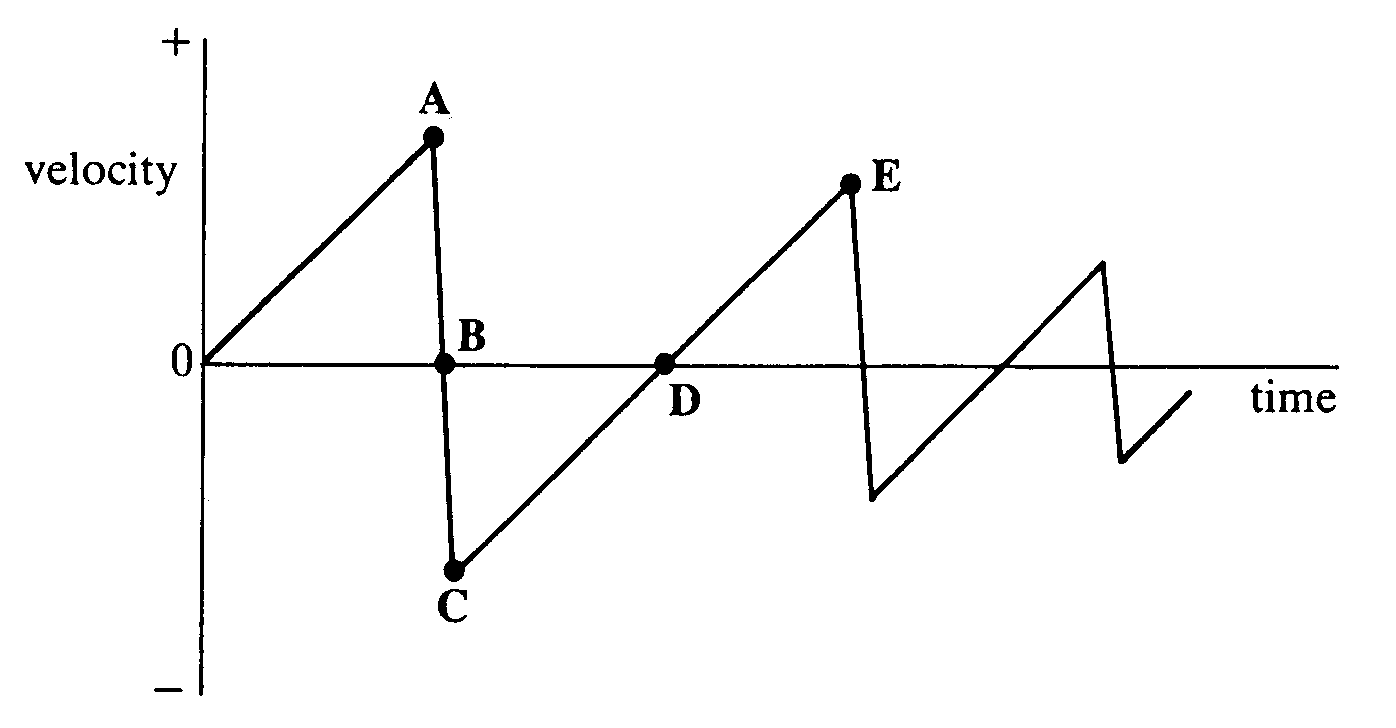
\includegraphics[width=\textwidth]{tennis.png}
\end{minipage}
\end{tabular}

\item
An air-track vehicle moves freely to and fro along an air track, colliding elastically with the buffers at each end of the track. Which one of the graphs below best represents how the acceleration of the vehicle varies with time?

\vspace{-15pt}
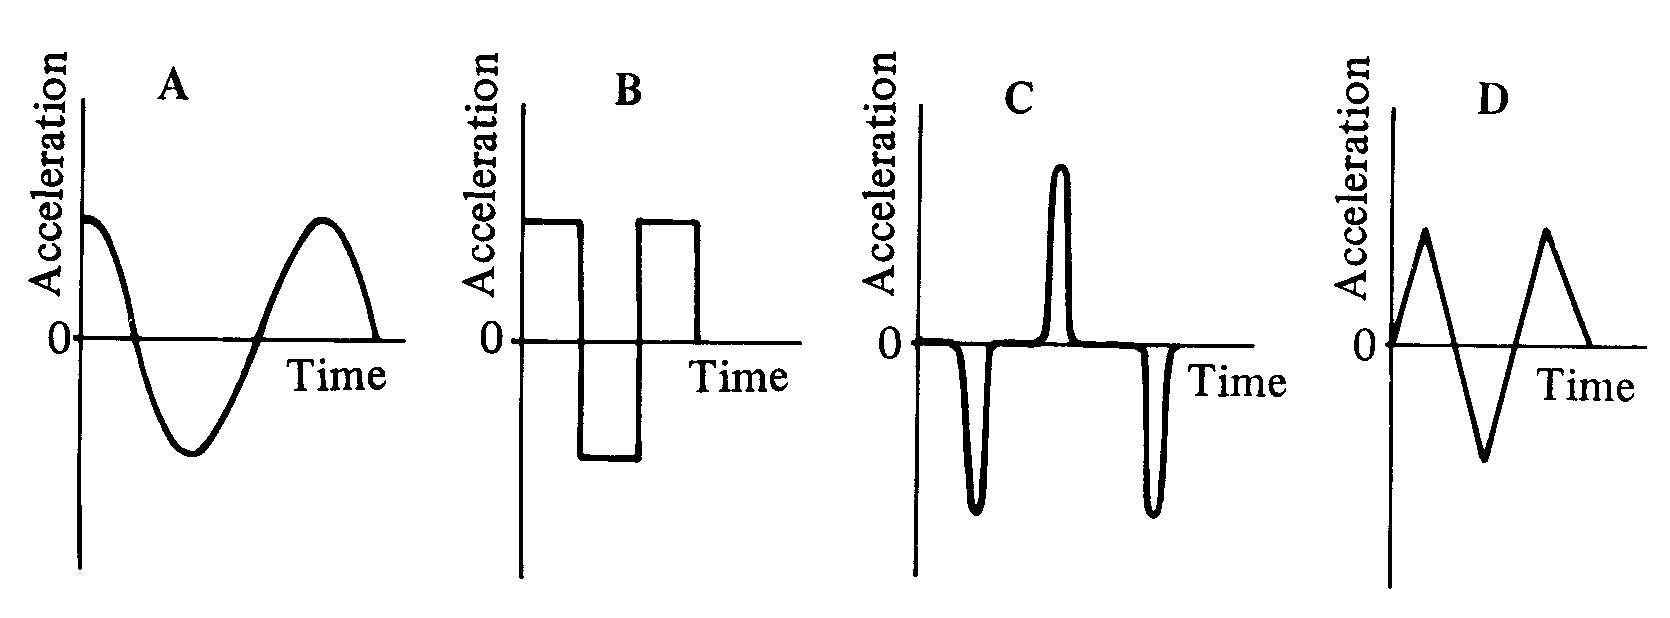
\includegraphics[width=0.9\textwidth]{airtrack.png}
\vspace{-20pt}
\begin{enumerate}
\setcounter{enumii}{4}
\item Either (b) or (d) depending on the mass of the vehicle
\end{enumerate}

\item
An Olympic ice skater starts a slow spin on her ice skates. As she brings her arm and free leg closer to her axis of rotation, she spins faster. Which one of the following statements must be true?
\begin{enumerate}
\item Angular momentum remains constant but rotational kinetic energy increases.
\item Angular momentum increases but rotational kinetic energy remains the same.
\item Both angular momentum and rotational kinetic energy increase.
\item Both angular momentum and rotational kinetic energy remain the same.
\item Any of the above might be true depending on the type of spin.
\end{enumerate}

\item
A stone of mass 0.1 kg is projected with velocity 10 m/s from a point P as shown in the following diagram. Neglecting the air resistance, the magnitude of the change in momentum between leaving P and arriving at Q is

\begin{tabular}{l r}

\begin{minipage}{0.5\textwidth}
\begin{enumerate}
\item zero.
\item 1/2 m/s.
\item 1 kg$\,\cdot\,$m/s.
\item 2 kg$\,\cdot\,$m/s.
\item $\sqrt{2}$ kg$\,\cdot\,$m/s.
\end{enumerate}
\end{minipage} &
\begin{minipage}{0.4\textwidth}
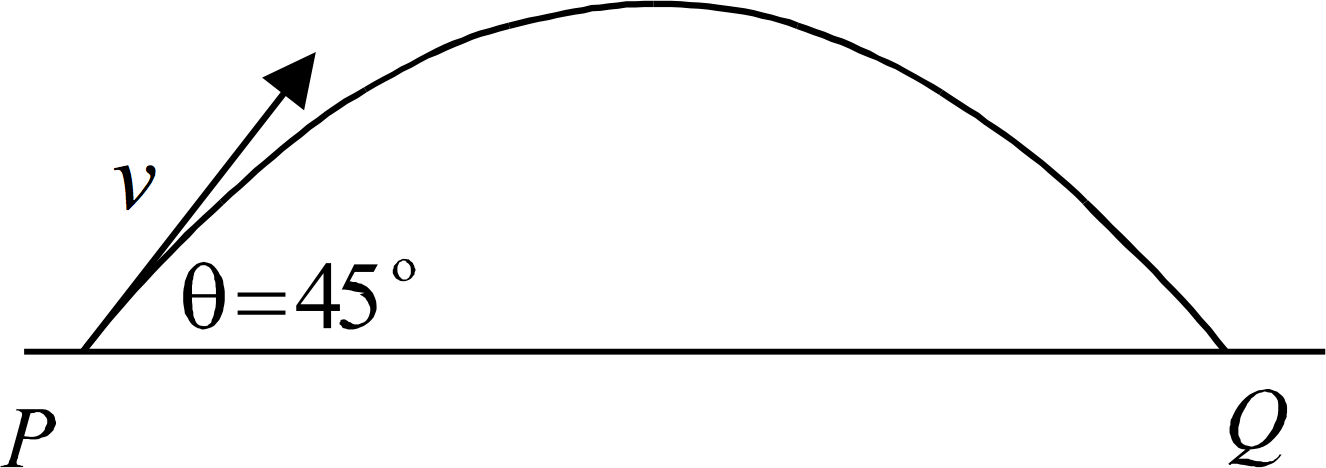
\includegraphics[width=\textwidth]{momentum.png}
\end{minipage}
\end{tabular}

\item
Two identical bowling balls A and B are each dropped from rest from the top of a tall tower as shown below. Ball A is dropped 2.0 s before ball B is dropped but both balls fall for some time before ball A strikes the ground. Air resistance can be considered negligible during the fall. Consider the following statements:
\begin{enumerate}[label=\Roman*.]
\item At the moment ball B is released, ball A is traveling at about 10 m/s.
\item At the moment ball B is released, ball A has more mechanical energy than ball B.
\item At the moment ball B is released, ball A has the same mechanical energy as ball B.
\item After ball B is dropped but before ball A strikes the ground, the distance between the two balls remains constant.
\item After ball B is dropped but before ball A strikes the ground, the velocity of ball A with respect to ball B remains constant.
\end{enumerate}

\begin{tabular}{l r}

\begin{minipage}{0.775\textwidth}
Which of the above statements are correct?
\begin{enumerate}
\item I only
\item II and V
\item III and V
\item I, III, and V
\item I, II, III, IV, and V
\end{enumerate}
\end{minipage} &
\begin{minipage}{0.125\textwidth}
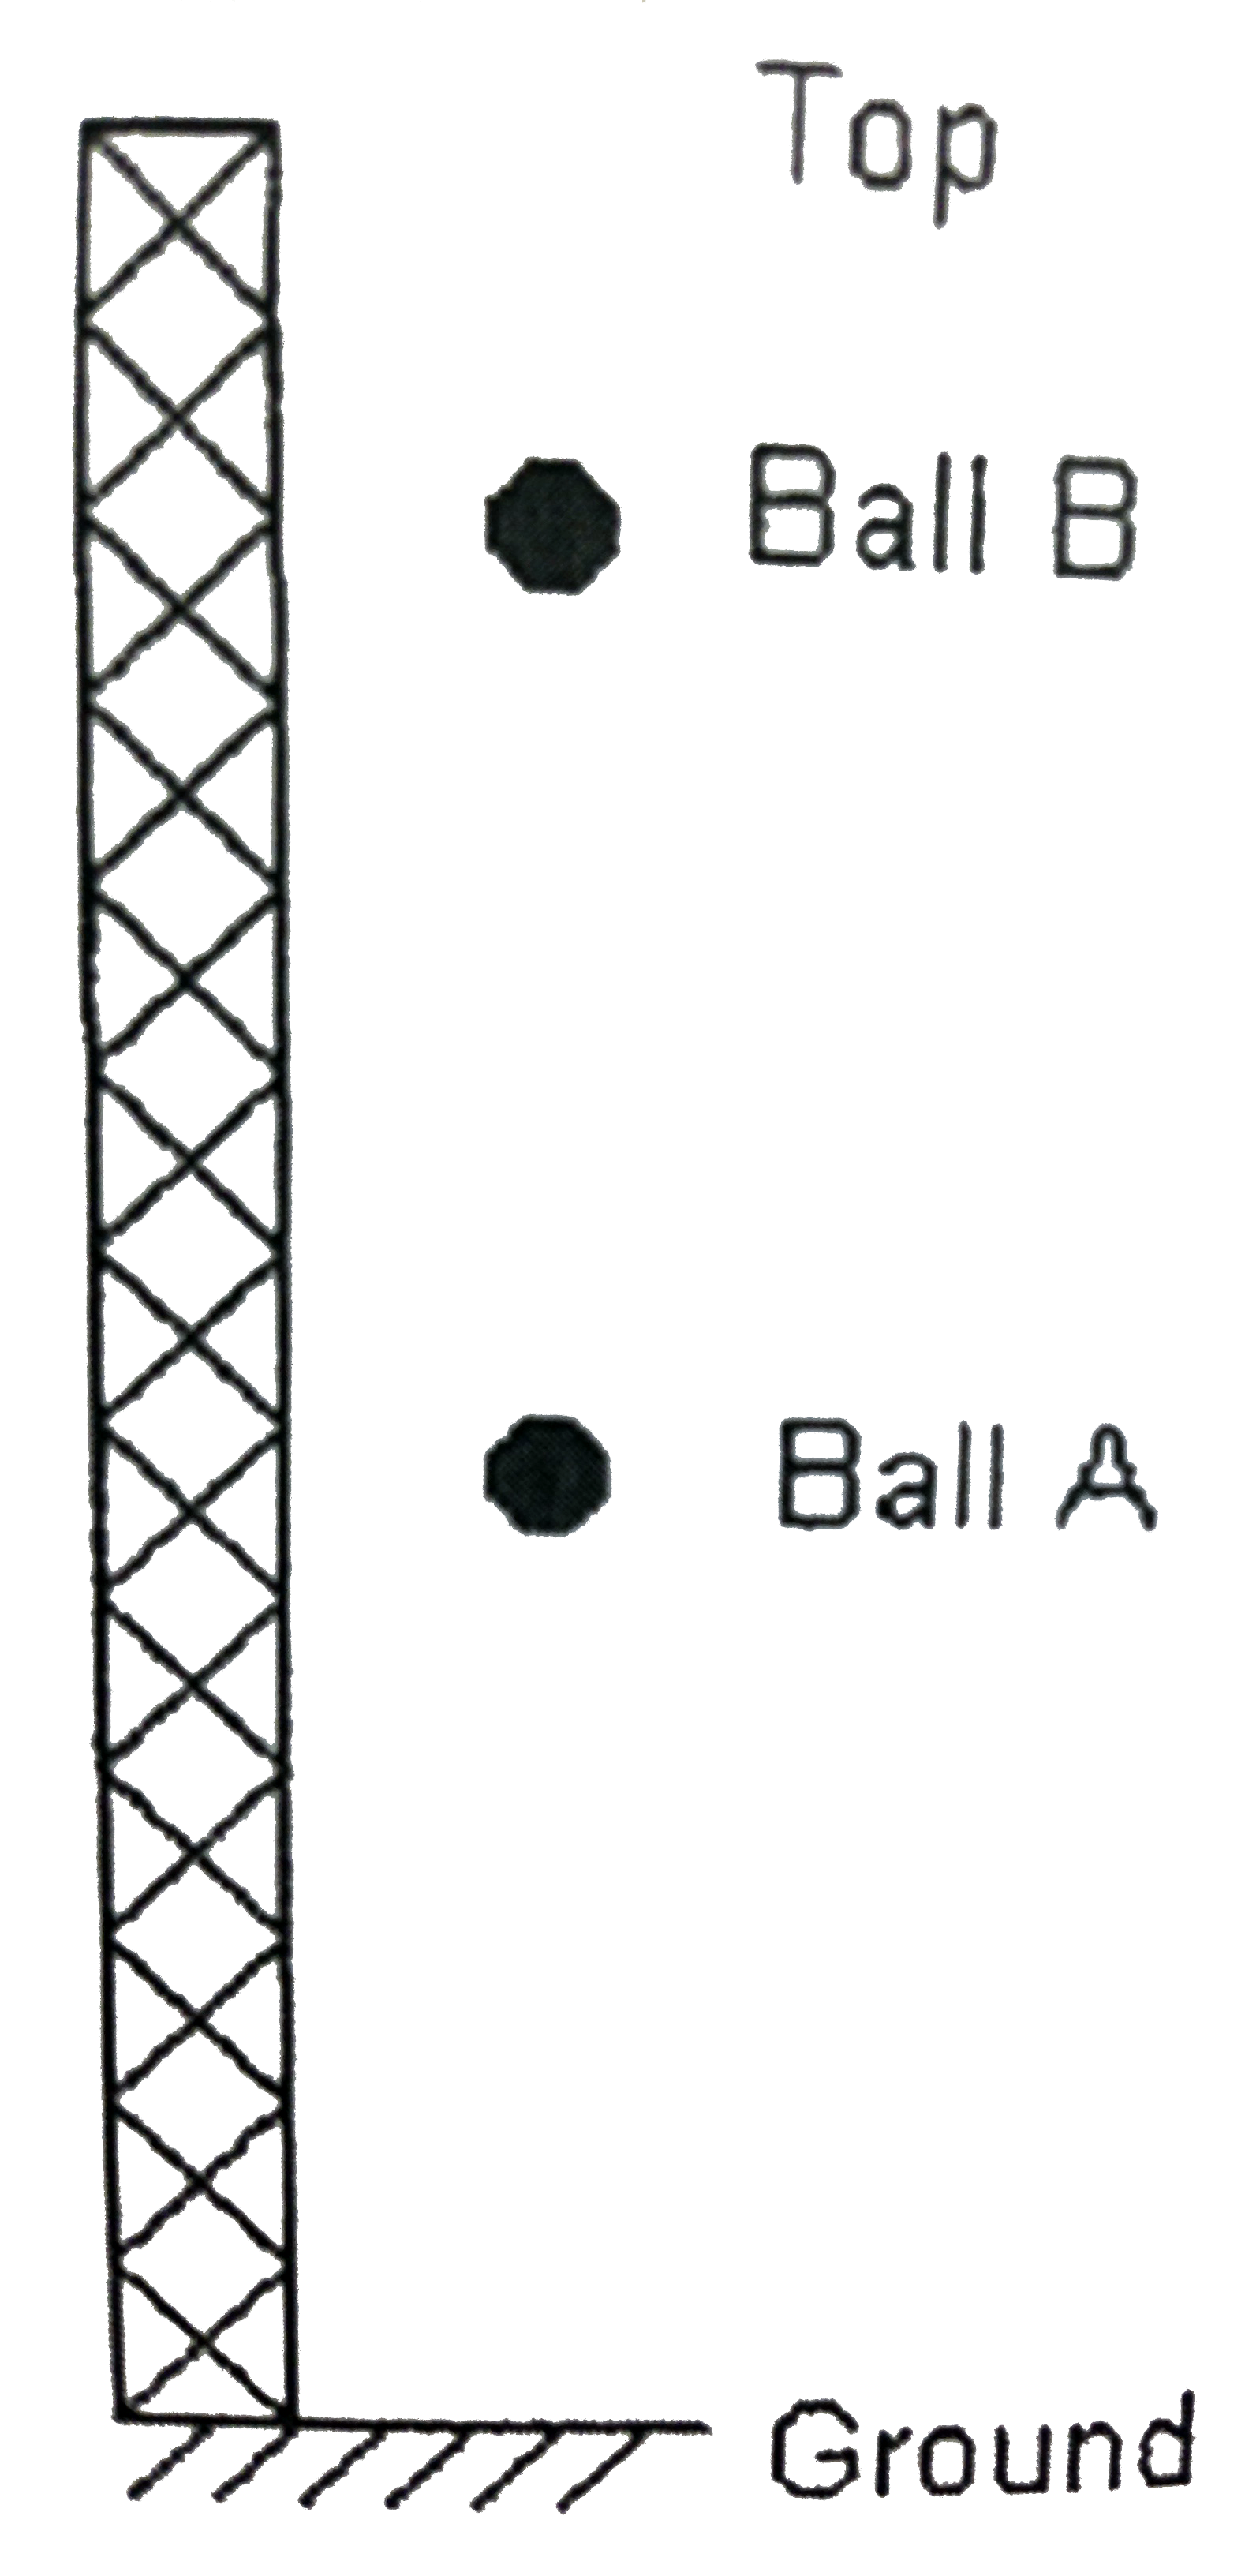
\includegraphics[width=\textwidth]{tower.png}
\end{minipage}
\end{tabular}

\item
A, B, C, and D are points on a vertical straight line such that AB = BC = CD. If a body is released from position A at rest, the times of descent through AB, BC, and CD, respectively, are in the ratio
\begin{enumerate}
\item $1:\sqrt{3}-\sqrt{2}:\sqrt{3}+\sqrt{2}$
\item $1:\sqrt{2}-1:\sqrt{3}-\sqrt{2}$
\item $1:\sqrt{2}-1:\sqrt{3}$
\item $1:\sqrt{2}:\sqrt{3}-1$
\item $1:\sqrt{2}:\sqrt{3}$
\end{enumerate}

\item
A projectile is launched at an angle above a flat ground such that it reaches a maximum horizontal distance $R$. The maximum height that the projectile rises is $H$. Air resistance is negligible. What is the ratio $H/R$?
\begin{enumerate}
\item 1
\item 2
\item 1.5
\item 0.5
\item 0.25
\end{enumerate}

\item
Car A ran the red light and hit Car B which had the right of way at the intersection. Car A was more severely damaged than Car B, but fortunately no one was injured. You are to investigate the accident and decide which of the following statements are correct.
\begin{enumerate}
\item The driver of Car A was at fault because Car A collided with Car B before Car B collided with Car A.
\item The driver of Car A was at fault even though both cars collided at the same moment.
\item Both drivers were at fault because both cars collided at the same moment.
\item The driver of Car B was at fault because Car B exerted more force on Car A, and, as a result, Car A was damaged more.
\item The driver of Car A was at fault because being the initiator Car A exerted more force on Car B.
\end{enumerate}

\item
A ball attached to a rope is twirled around a stick of diameter $a$ as shown in the diagram. Ignore gravity and friction. What quantities are conserved in the motion of the ball?

\begin{tabular}{l r}

\begin{minipage}{0.6\textwidth}
\begin{enumerate}
\item Mechanical energy
\item Momentum
\item Angular momentum
\item Mechanical energy and angular momentum
\item Momentum and angular momentum
\end{enumerate}
\end{minipage} &
\begin{minipage}{0.3\textwidth}
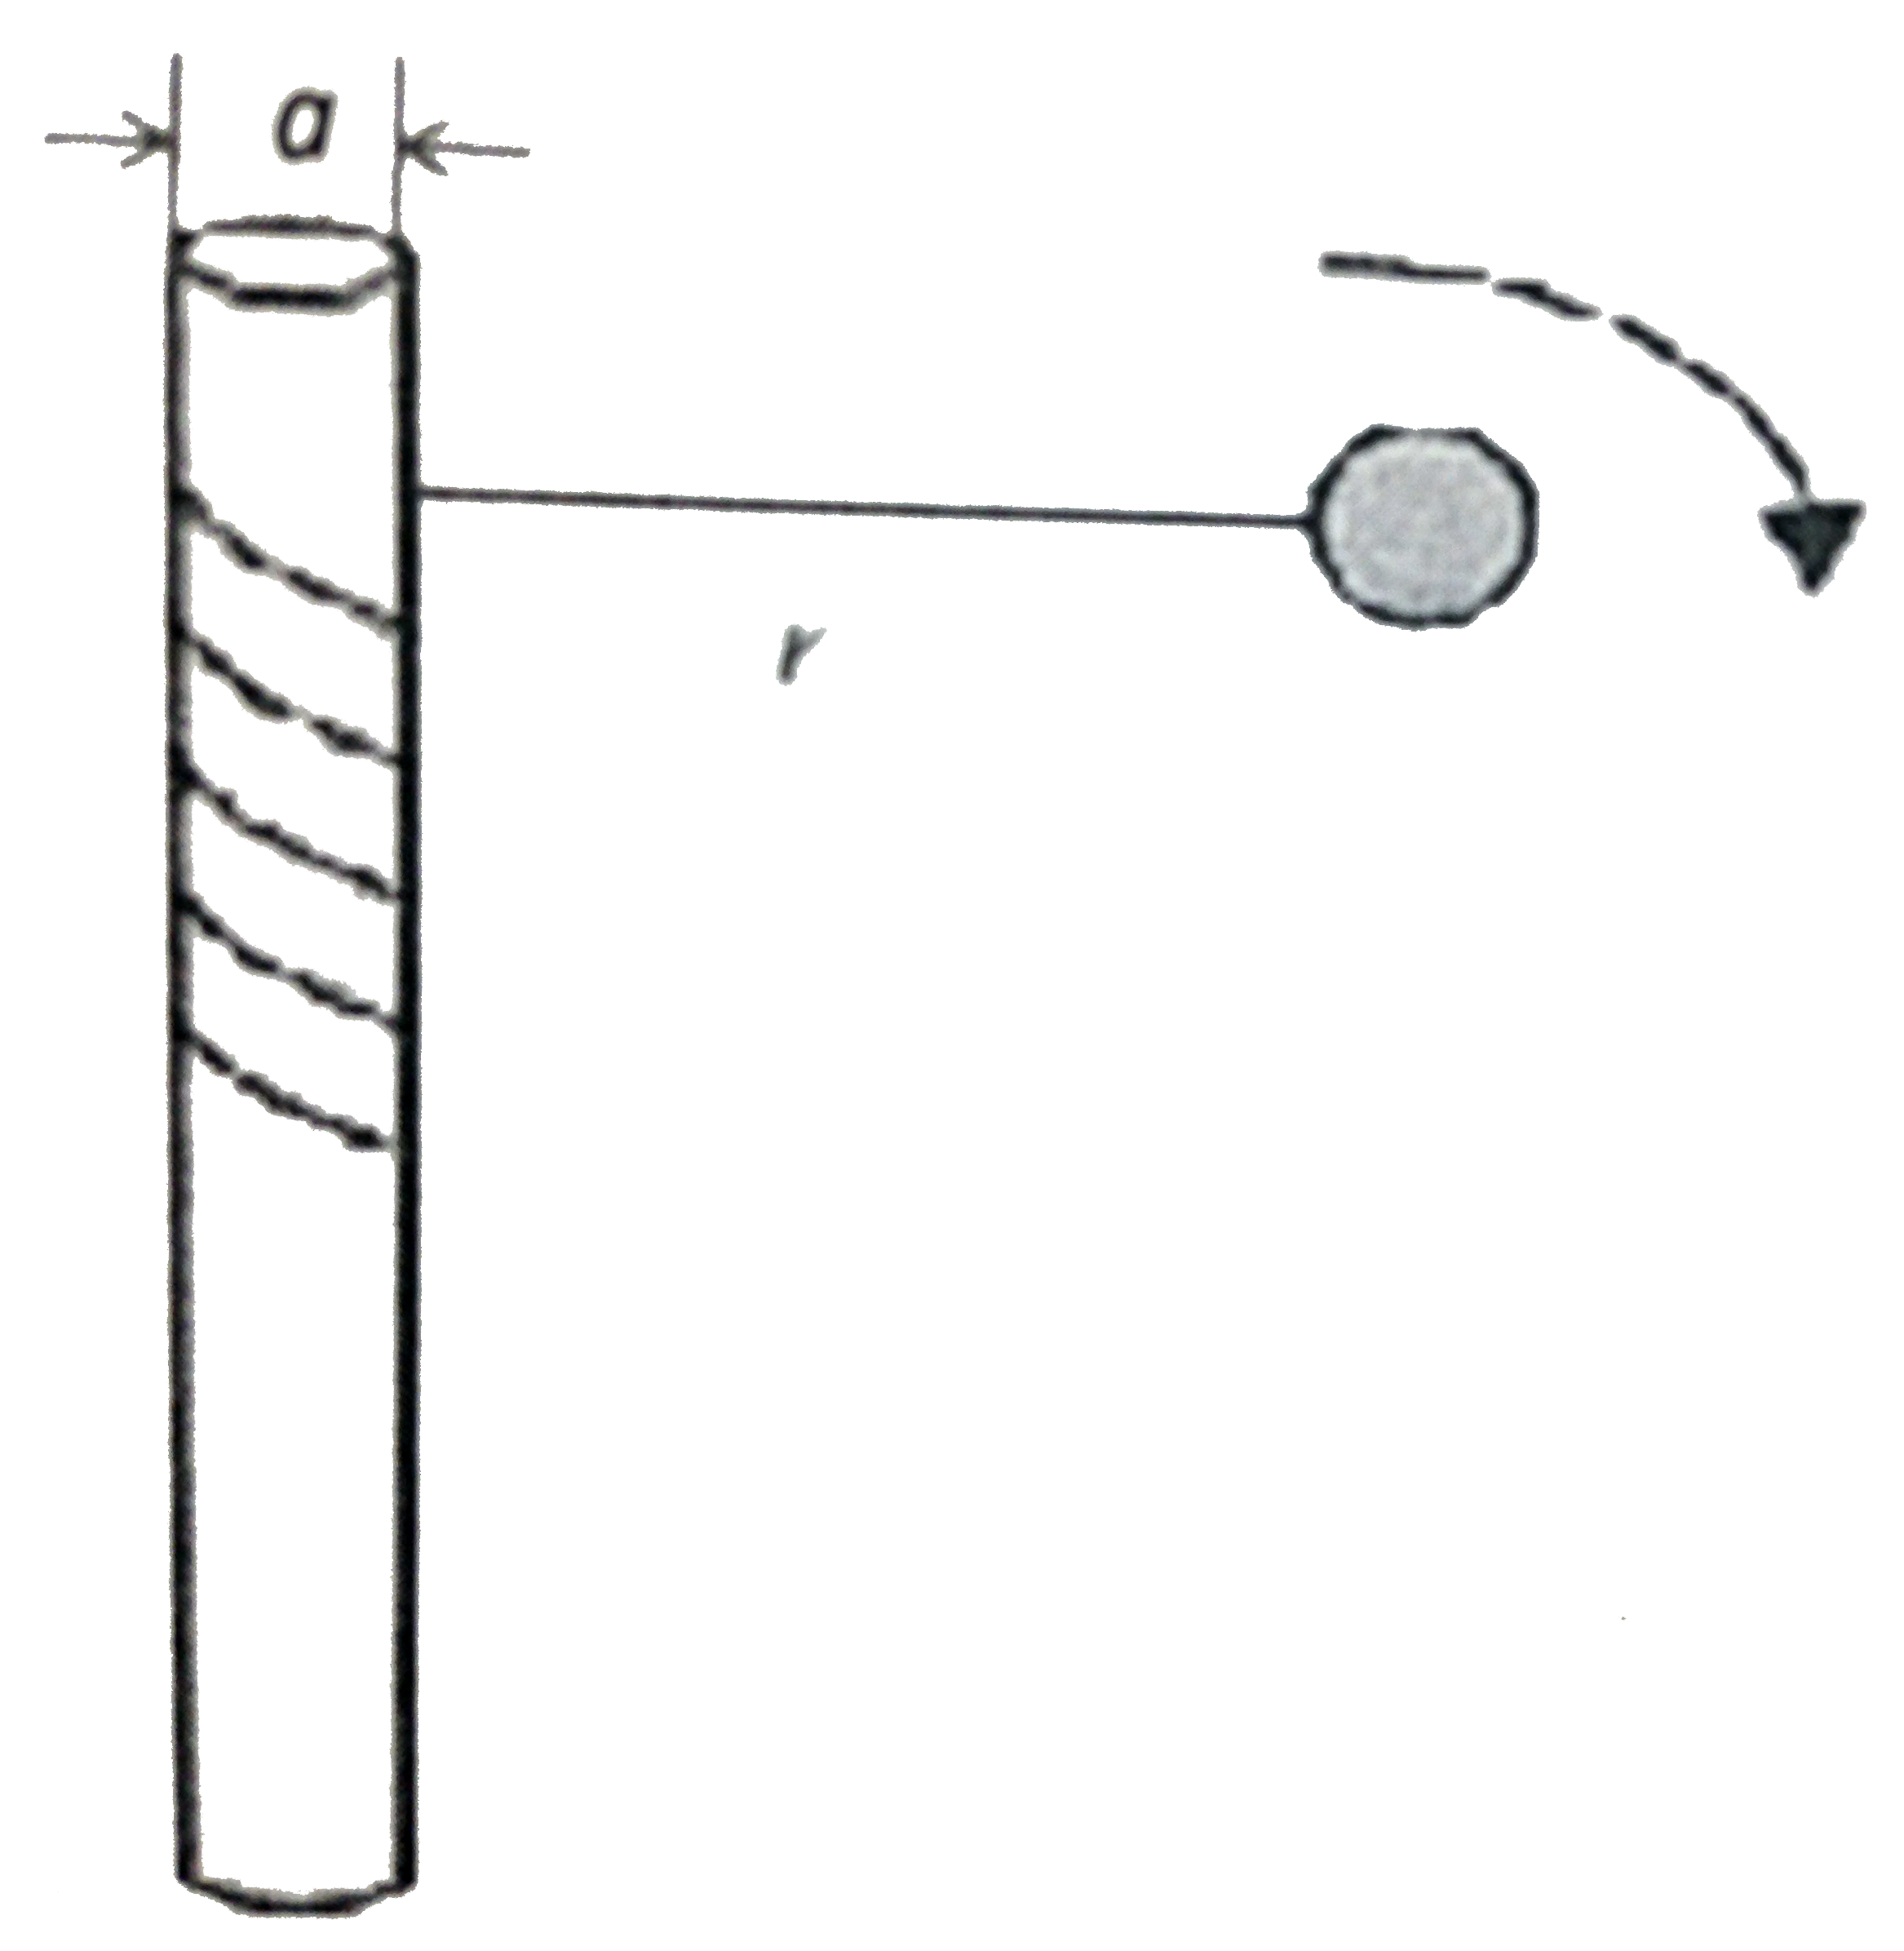
\includegraphics[width=\textwidth]{twirl.png}
\end{minipage}
\end{tabular}

\item
The period of a simple pendulum on the ground is 1 s. If it is placed on a satellite on a circular orbit around Earth at 100 km above the ground, its period will be approximately
\begin{enumerate}
\item 11.2 s.
\item 1 s.
\item 2.45 s.
\item 0.
\item $\infty$.
\end{enumerate}

\vfill
\newpage

\begin{tabular}{l r}

\begin{minipage}[b]{0.5\textwidth}
\item
A small mass $m$ is moved from either position A or B to where it is on the figure. Positions A and B are equidistant from a large mass $M$. Mass $m$ starts at rest and ends at rest. Which of the following is true regarding the energy required to move mass $m$ from its initial position? Neglect resistive forces.
\end{minipage} &
\begin{minipage}[b]{0.4\textwidth}
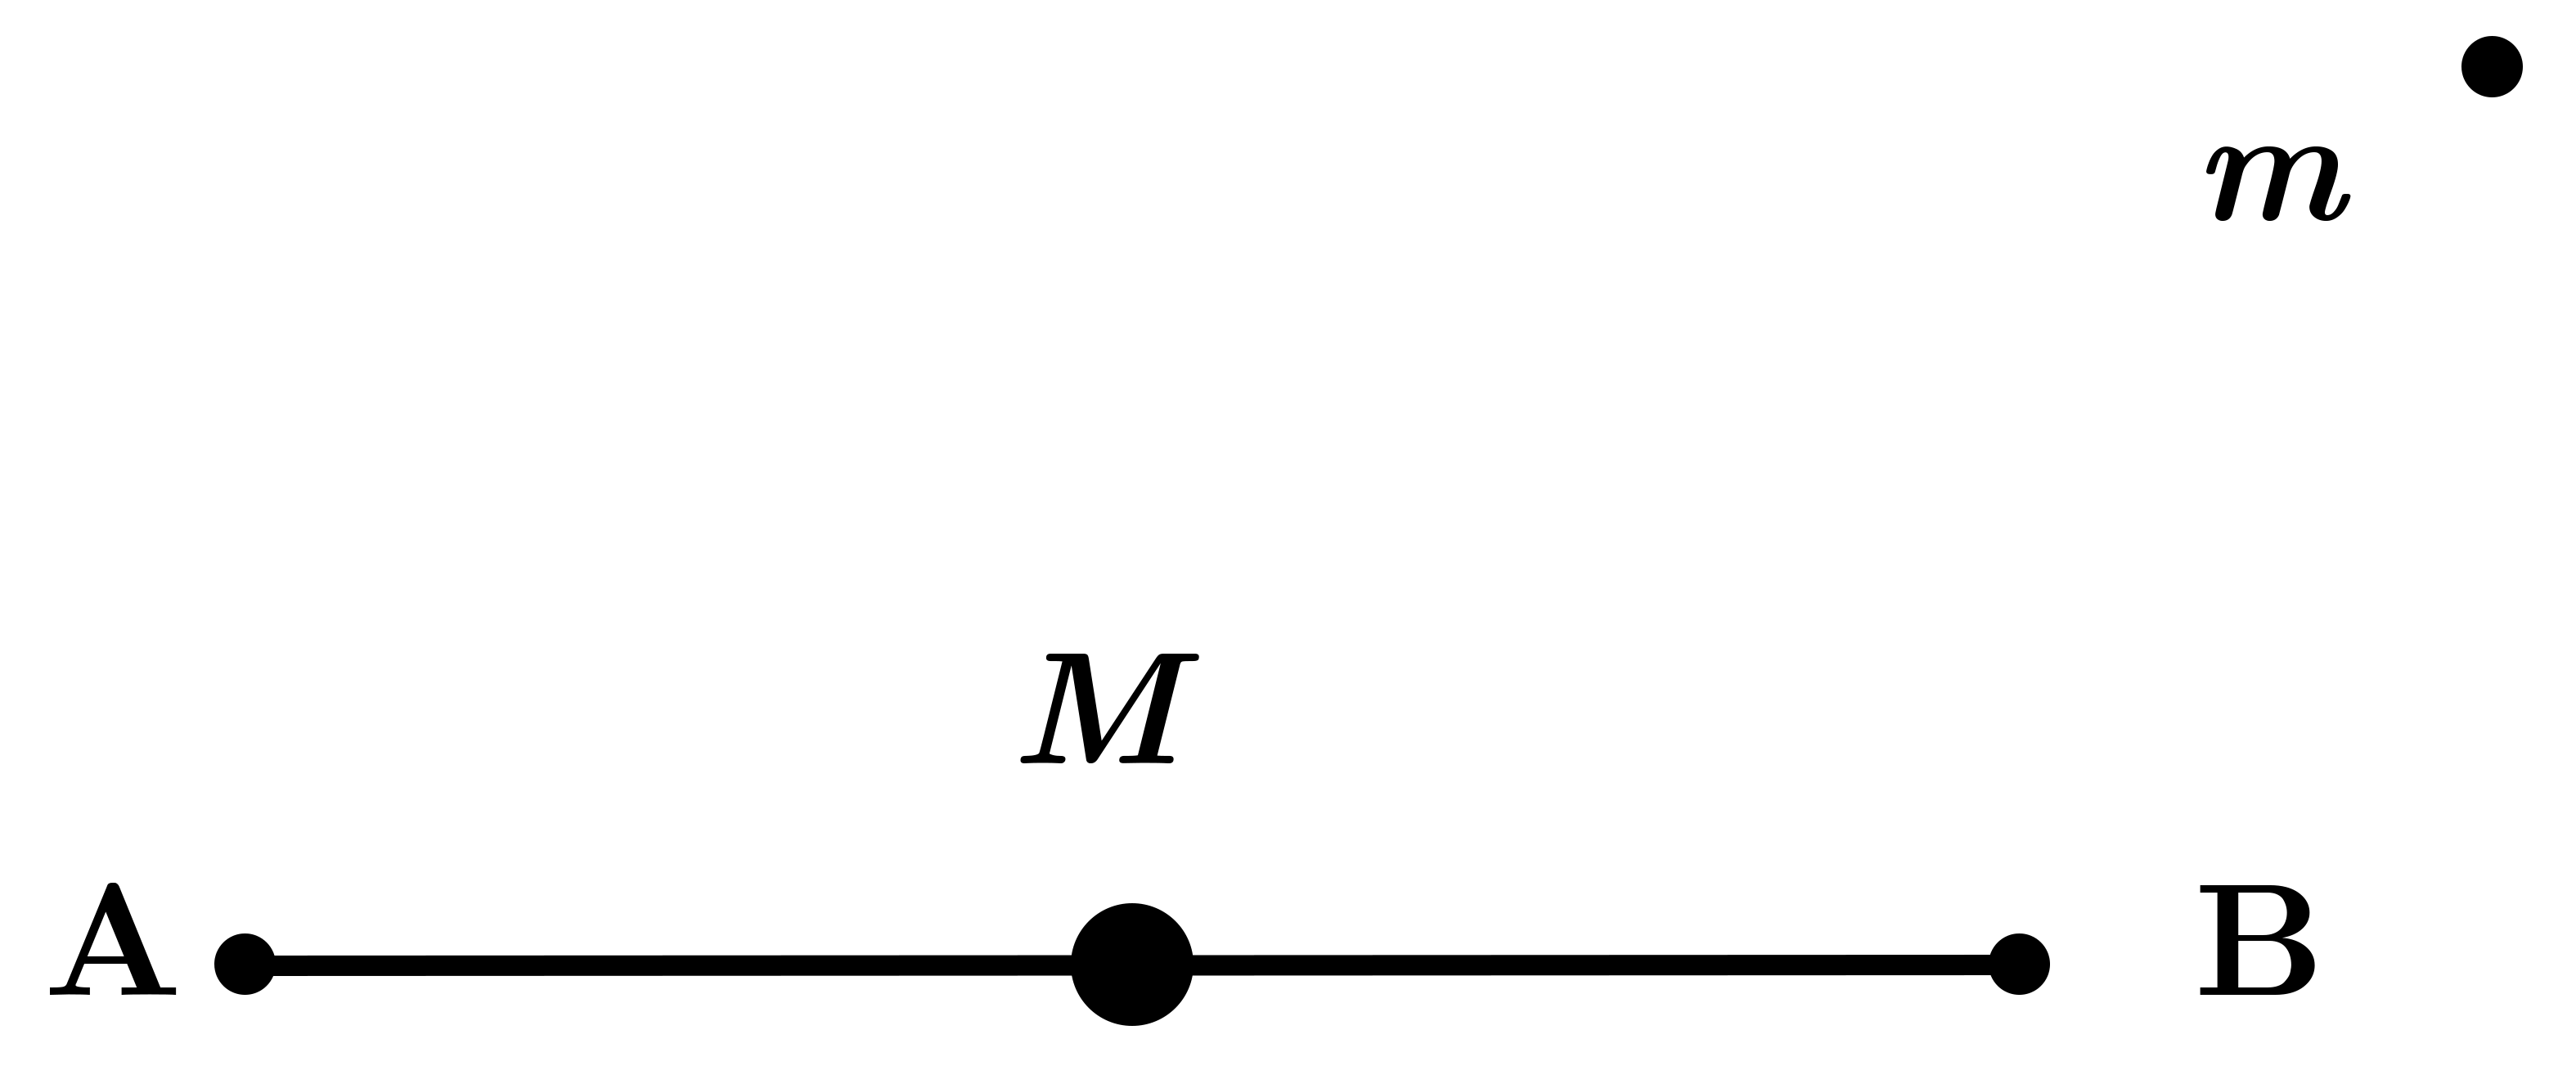
\includegraphics[width=\textwidth]{move.png}
\end{minipage}
\end{tabular}
\begin{enumerate}
\item It takes less energy to move it from A because the distance is longer but the force is attractive.
\item It takes less energy to move it from B because the distance is less.
\item It takes the same amount of energy to move the mass from A and from B.
\item There is not enough information to answer the question because the answer depends on the path taken by mass $m$.
\item There is not enough information to answer the question because the answer depends on the velocity of the mass as it moves.
\end{enumerate}

\item
As shown in the figure a yo-yo is released form hand with the string wrapped around the finger. Let $g$ be the acceleration of gravity. If the hand is held still, the magnitude and direction of the acceleration of the yo-yo is

\begin{tabular}{l r}

\begin{minipage}{0.8\textwidth}
\begin{enumerate}
\item less than $g$, downward.
\item less than $g$, upward.
\item $g$, downward.
\item greater than $g$, upward.
\item greater than $g$, downward.
\end{enumerate}
\end{minipage} &
\begin{minipage}{0.1\textwidth}
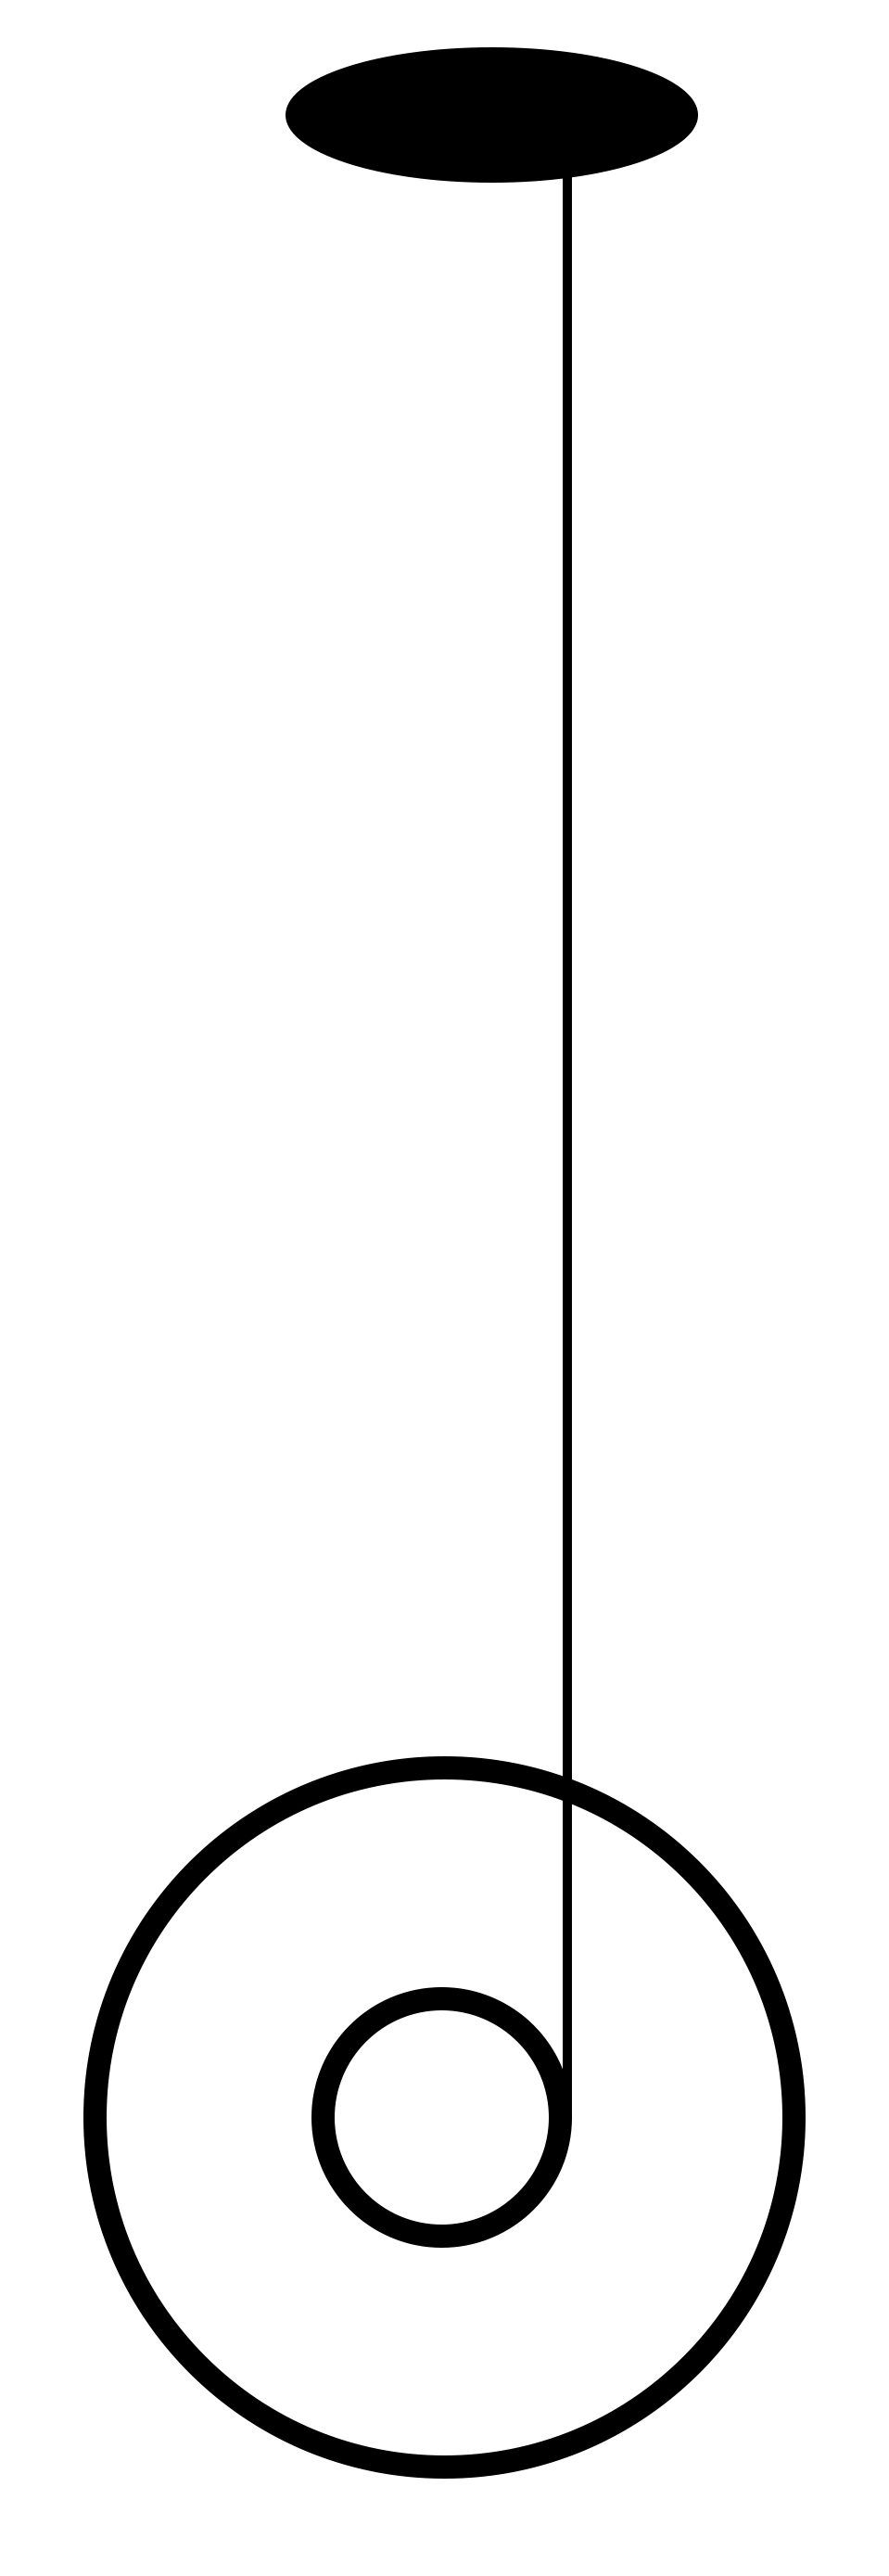
\includegraphics[width=\textwidth]{yoyo.png}
\end{minipage}
\end{tabular}

\item
Three blocks (A, B, and C) initially at rest are each pushed by equal forces, $F$, frictionlessly across a horizontal surface for a distance of 2 meters. The mass of block A is greater than block B, and the mass of block B is greater than block C.\\
Which of the blocks will have received the greatest impulse during the two meter push?

\begin{tabular}{l r}

\begin{minipage}{0.4\textwidth}
\begin{enumerate}
\item Block A
\item Block B
\item Block C
\item All blocks will have received the same impulse
\item It depends on the actual masses of the blocks
\end{enumerate}
\end{minipage} &
\begin{minipage}{0.5\textwidth}
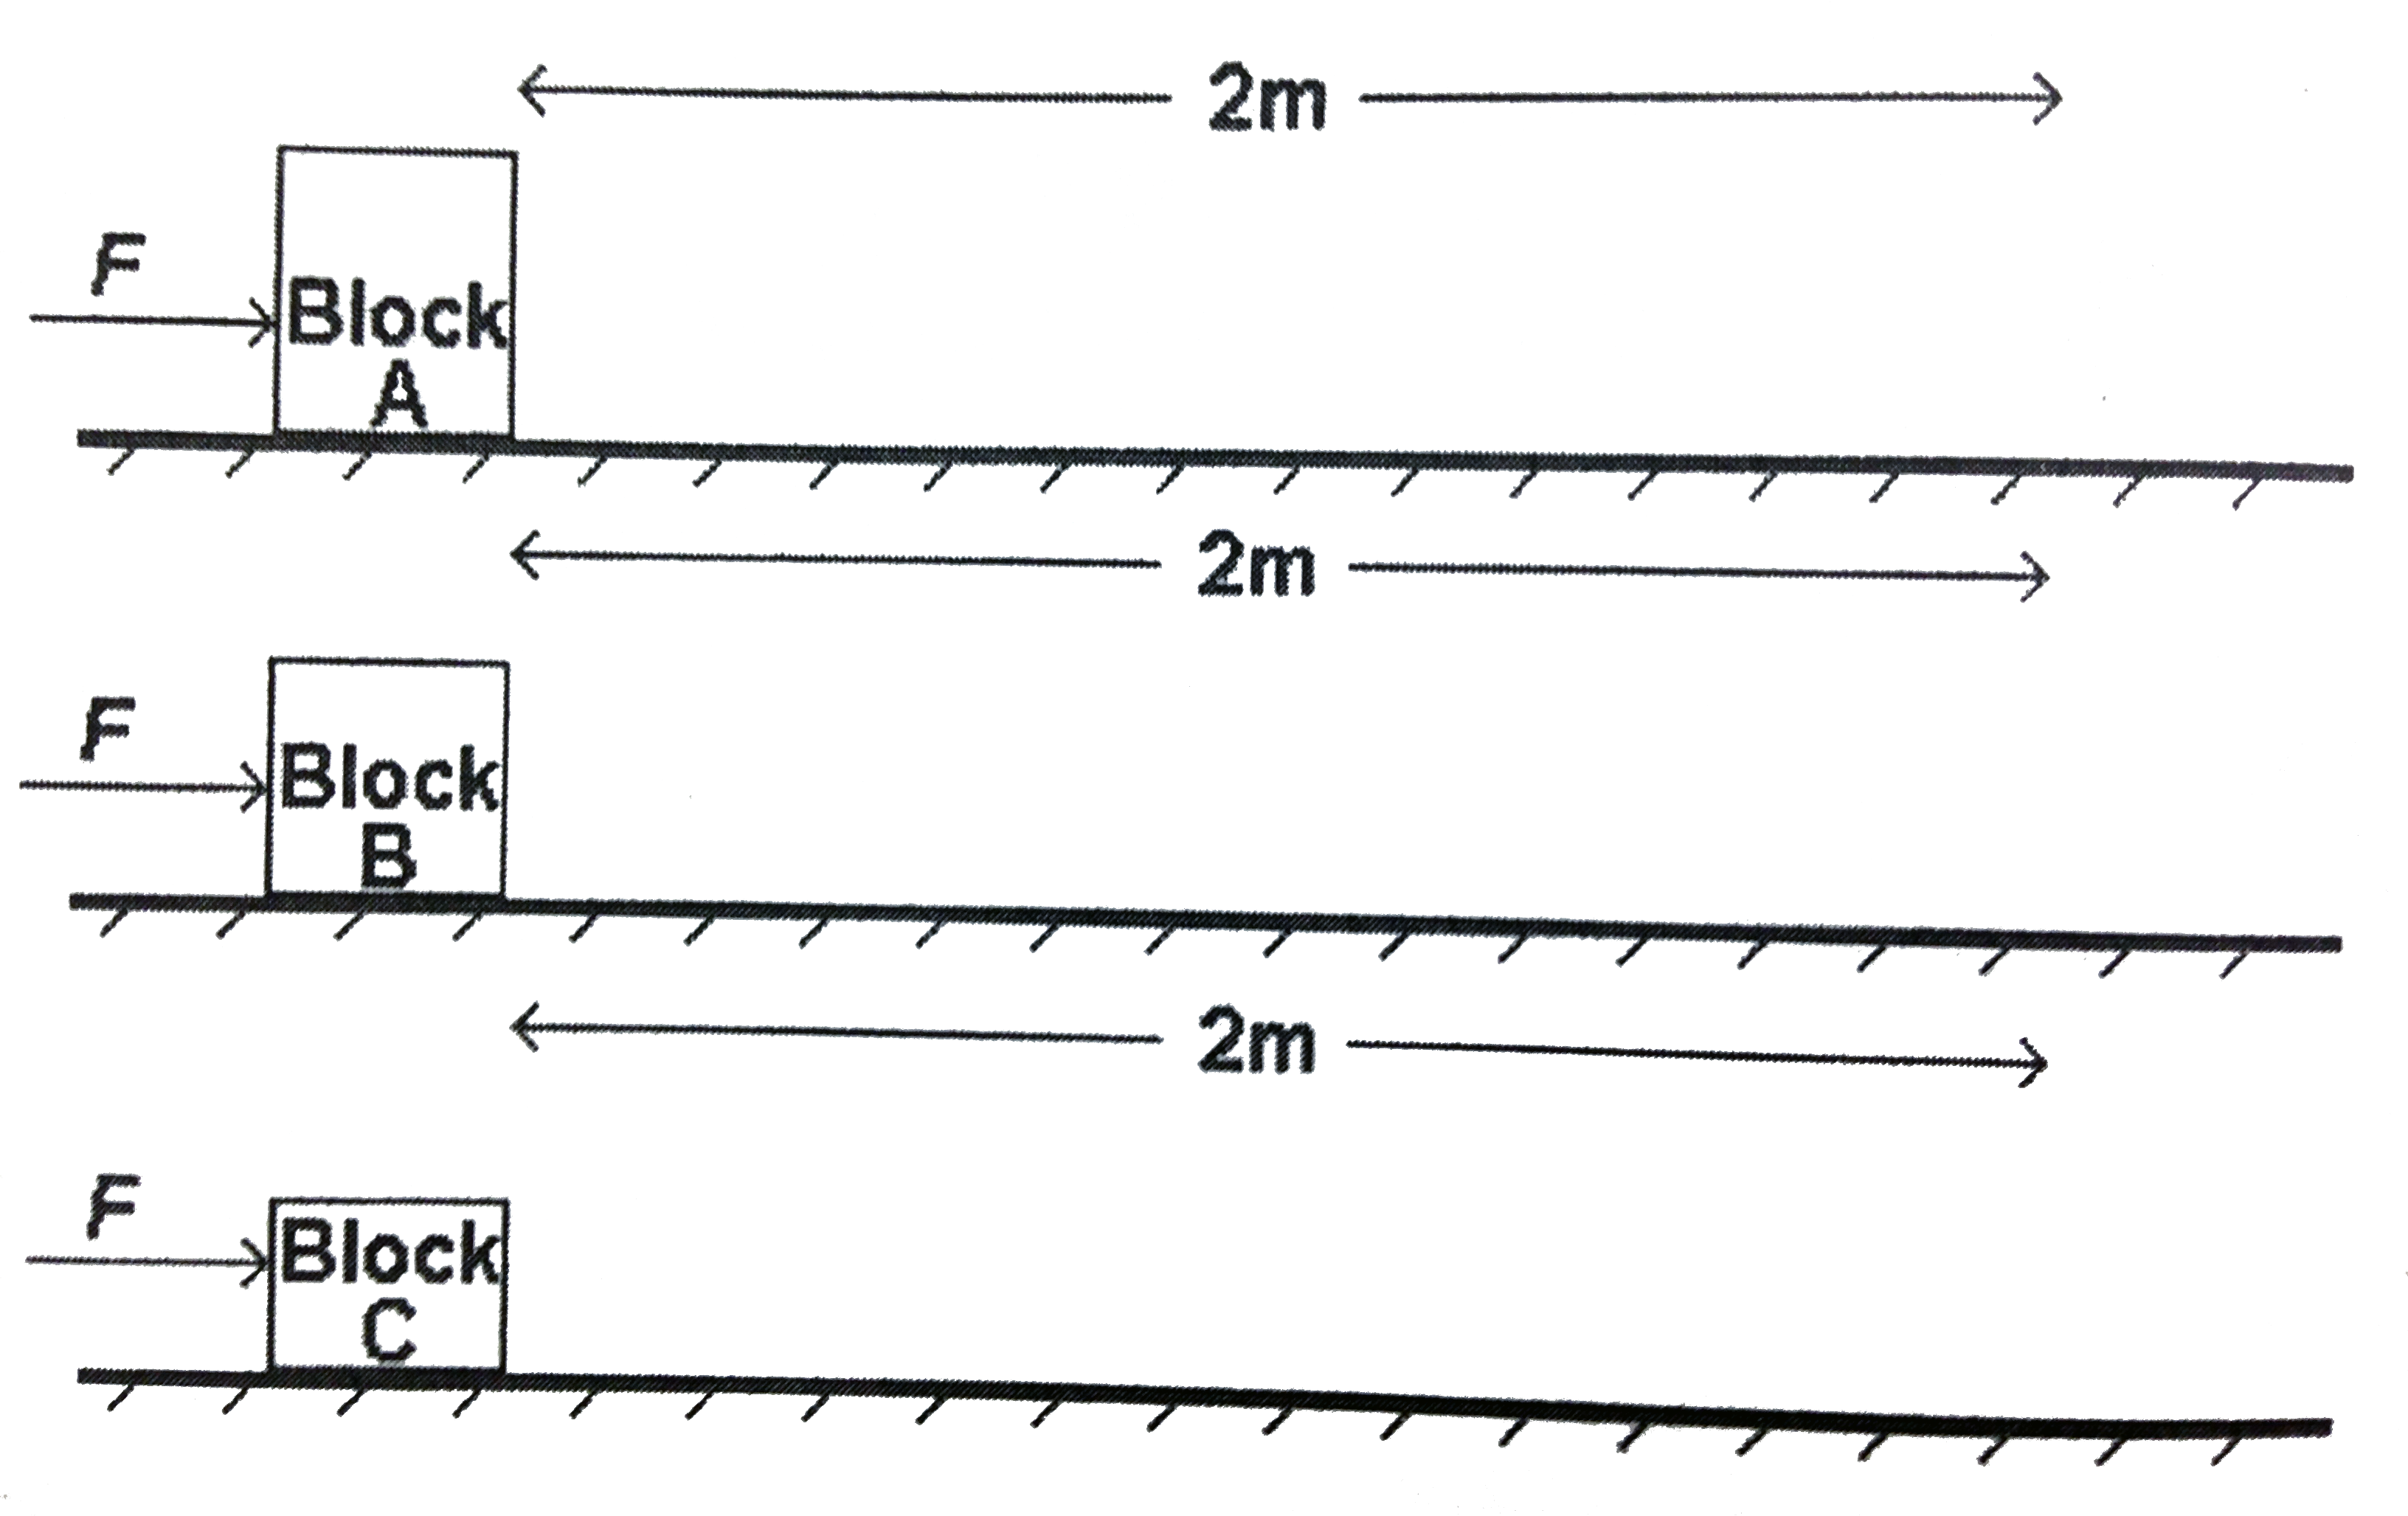
\includegraphics[width=\textwidth]{impulse.png}
\end{minipage}
\end{tabular}

\item
A hose is ejecting water out horizontally at a constant rate of 0.8 kg/s, which hits a wooden block of mass 1.2 kg on a horizontal support. The friction between the block and the support is 1.8 N. Calculate the speed of the water coming out from the hose if the block moves with constant acceleration of 0.5 m/s$^2$. Assume that the vertical speed of the water and its speed after hitting the block are negligible.

\begin{tabular}{l r}

\begin{minipage}{0.5\textwidth}
\begin{enumerate}
\item 1.5 m/s
\item 2.25 m/s
\item 3 m/s
\item 5 m/s
\item 6 m/s
\end{enumerate}
\end{minipage} &
\begin{minipage}{0.4\textwidth}
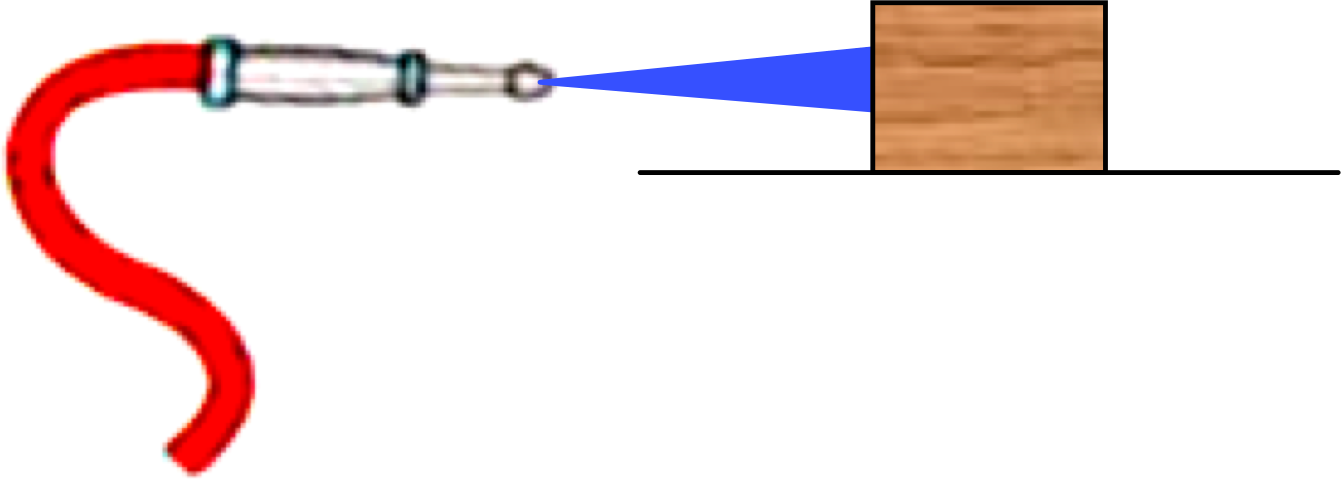
\includegraphics[width=\textwidth]{hose.png}
\end{minipage}
\end{tabular}

\item
A uniform chain of mass $m$ and length $L$ is originally placed mid-way on the top of a fixed smooth double-sided wedge (Figure A). The length of each side of the wedge is $L$. It is then given a slight push. Find the kinetic energy of the chain when the whole chain has just slid to the left side of the wedge (Figure B).

\begin{tabular}{l r}

\begin{minipage}{0.3\textwidth}
\begin{enumerate}
\item $mgL\sin\theta$
\item $\displaystyle \frac{1}{2}mgL\sin\theta$
\item $\displaystyle \frac{1}{4}mgL\sin\theta$
\item $\displaystyle \frac{1}{8}mgL\sin\theta$
\item $2mgL\sin\theta$
\end{enumerate}
\end{minipage} &
\begin{minipage}{0.6\textwidth}
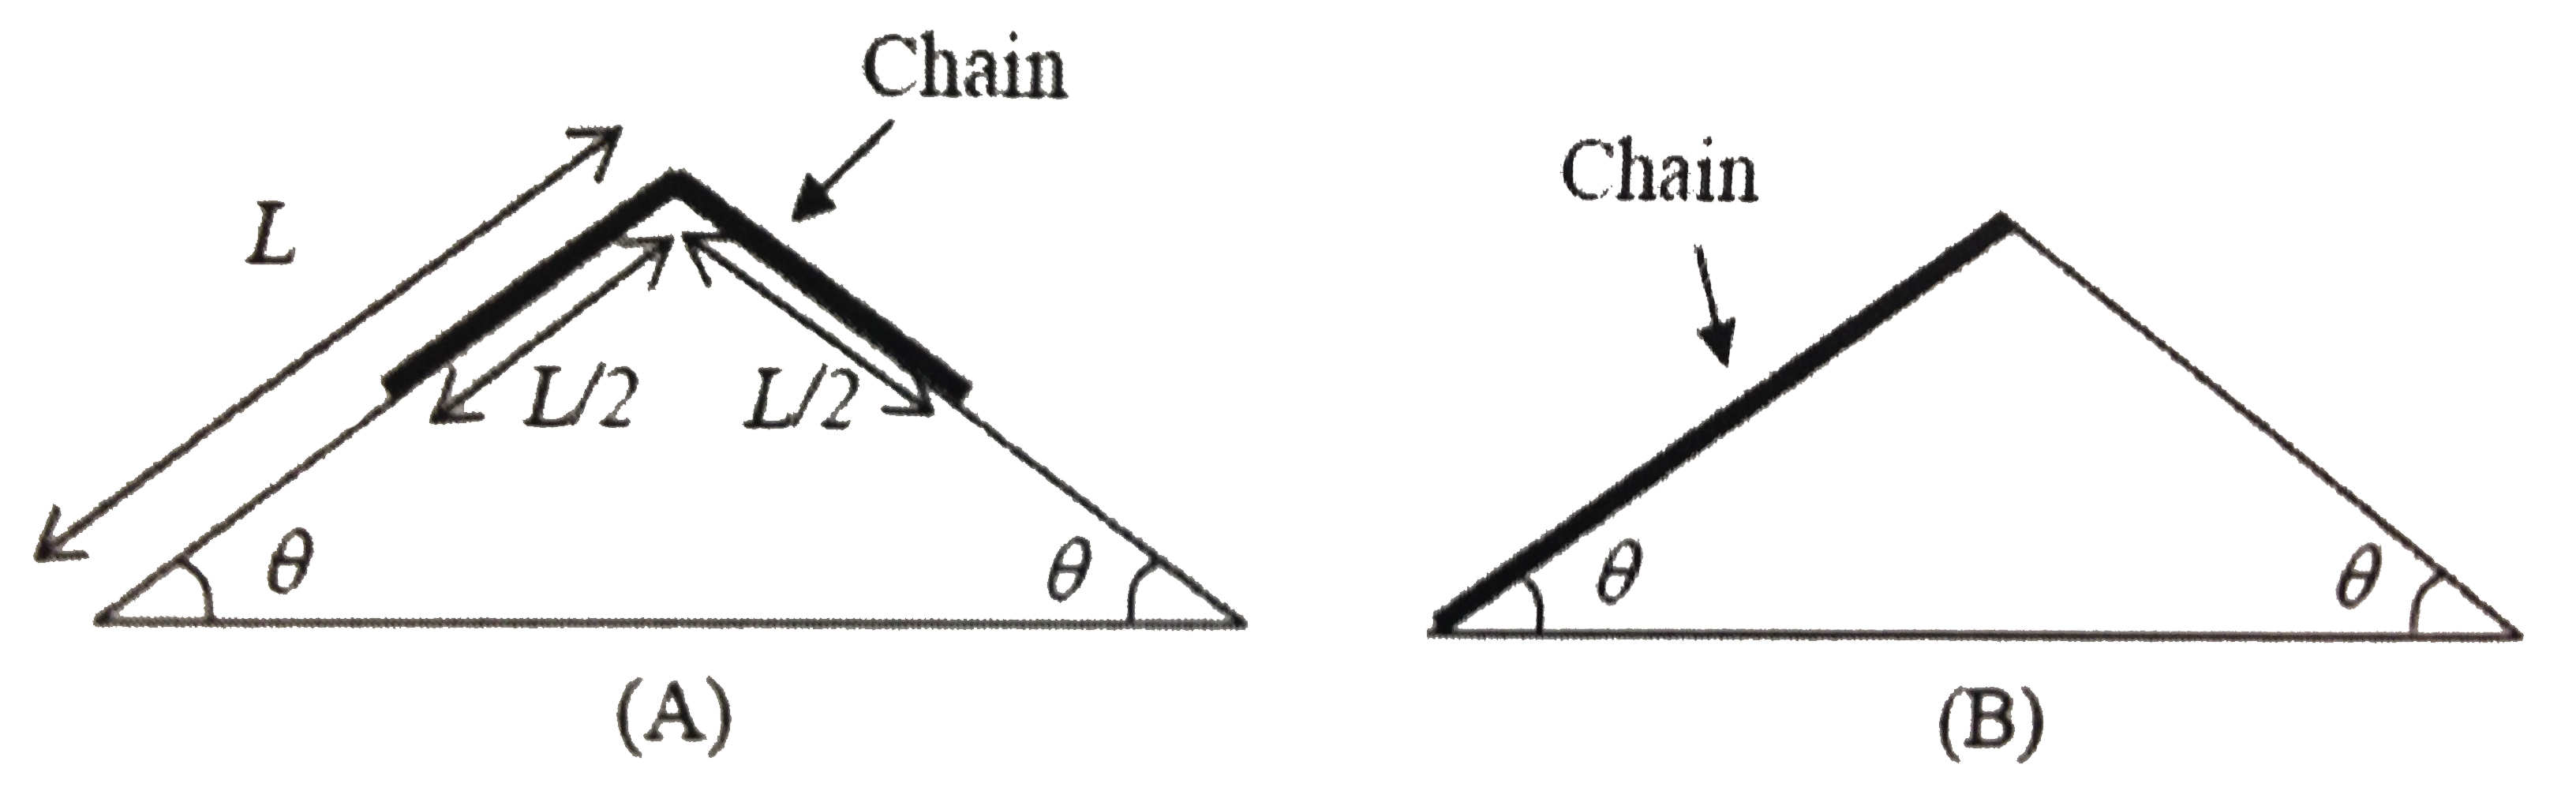
\includegraphics[width=\textwidth]{chain.png}
\end{minipage}
\end{tabular}

\item
On the long horizontal test track at Edwards AFB, both rocket and jet motors can be tested. On a certain day, a rocket motor, started from rest, accelerated constantly until its fuel was exhausted, after which it ran at constant speed. It was observed that this exhaustion of the rocket fuel took place as the rocket passed the midpoint of the measured test distance. Then a jet motor was started from rest down the track, with a constant acceleration for the entire distance. It was observed that both rocket and jet motors covered the test distance in exactly the same time. What was the ratio of the acceleration of the jet motor to that of the rocket motor?
\begin{enumerate}
\item $1:3$
\item $1:2$
\item $3:4$
\item $5:8$
\item $8:9$
\end{enumerate}

\vfill
\newpage

\item
The moment of inertia of a uniform sphere of mass $m$ and radius $R$ about its center of mass is $(2/5)mR^2$. The uniform sphere rotates at a fixed angular velocity on an axis through its center and has kinetic energy $E$. If the same sphere rotates at the same angular velocity about a parallel axis on the edge of the sphere, what is its kinetic energy?
\begin{enumerate}
\item $E/2$
\item $3E/2$
\item $5E/2$
\item $7E/2$
\item $9E/2$
\end{enumerate}

\item
A small block of mass 1 kg is projected upward along an inclined plane with an initial speed of $u = 2$ m/s. The angle of inclination of the inclined plane to the horizontal is $30\degree$; the kinetic friction and the maximum static friction between the small block and the inclined plane are the same and equal 6 N. Which of the following statements are correct?
\begin{enumerate}[label=\Roman*.]
\item The maximum height that the small block can reach is $h = 0.09$ m.
\item The small block will be momentarily at rest at the highest point and then moves down with a uniform acceleration.
\item The total mechanical energy of the small block will be lost against friction.
\end{enumerate}

\begin{tabular}{l r}

\begin{minipage}{0.5\textwidth}
\begin{enumerate}
\item I only
\item II only
\item I and II only
\item I and III only
\item I, II, and III
\end{enumerate}
\end{minipage} &
\begin{minipage}{0.4\textwidth}
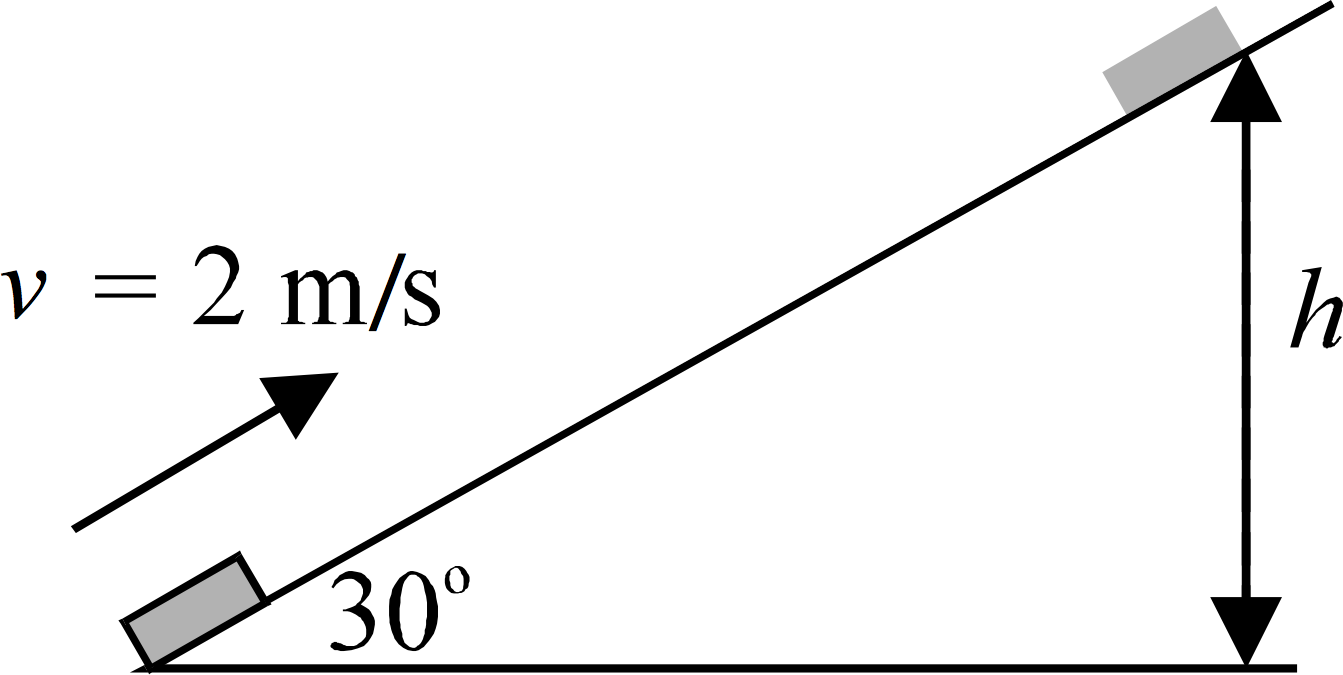
\includegraphics[width=\textwidth]{incline.png}
\end{minipage}
\end{tabular}

\item
An object of mass $m$ is attached to a spring. The restoring force of the spring is $F = -\lambda x^3$, where $x$ is the displacement. The oscillation period now depends on the oscillation amplitude. Suppose the object is initially at rest. If the initial displacement is $D$, then its period is $\tau$. If its initial displacement is $2D$, find the period. (\emph{Hint:} use dimensional analysis.)
\begin{enumerate}
\item $8\tau$
\item $2\tau$
\item $\tau$
\item $\tau/2$
\item $\tau/8$
\end{enumerate}

\vfill
\newpage

\item
A small point-like object is thrown horizontally off of a 40.0-m high building with an initial speed of 10.0 m/s. At any point along the trajectory there is an acceleration component tangential to the trajectory and an acceleration component perpendicular to the trajectory. How many seconds after the object is thrown is the tangential component of the acceleration of the object equal to three times the perpendicular component of the acceleration of the object? Ignore air resistance.
\begin{enumerate}
\item 4.00 s
\item 3.00 s
\item 2.00 s
\item 1.00 s
\item The building is not height enough for this to occur.
\end{enumerate}

\item
A compound pendulum is made of a light and rigid rod of length $L$ with one end attached to a hinge on the ceiling. A small ball of mass $m$ is attached to the other end of the rod, and another small ball of mass $2m$ is attached to the middle of the rod. Find the frequency of the simple harmonic oscillation of the pendulum.

\begin{tabular}{l r}

\begin{minipage}[t]{0.6\textwidth}
\begin{enumerate}
\item $\displaystyle \frac{1}{2\pi}\sqrt\frac{g}{2L}$
\item $\displaystyle \frac{1}{2\pi}\sqrt\frac{4g}{3L}$
\item $\displaystyle \frac{1}{2\pi}\sqrt\frac{3g}{2L}$
\item $\displaystyle \frac{1}{2\pi}\sqrt\frac{9g}{4L}$
\item $\displaystyle \frac{1}{2\pi}\sqrt\frac{9g}{2L}$
\end{enumerate}
\end{minipage} &
\begin{minipage}[b]{0.3\textwidth}
\raisebox{-\dimexpr+\height-\ht\strutbox\relax}{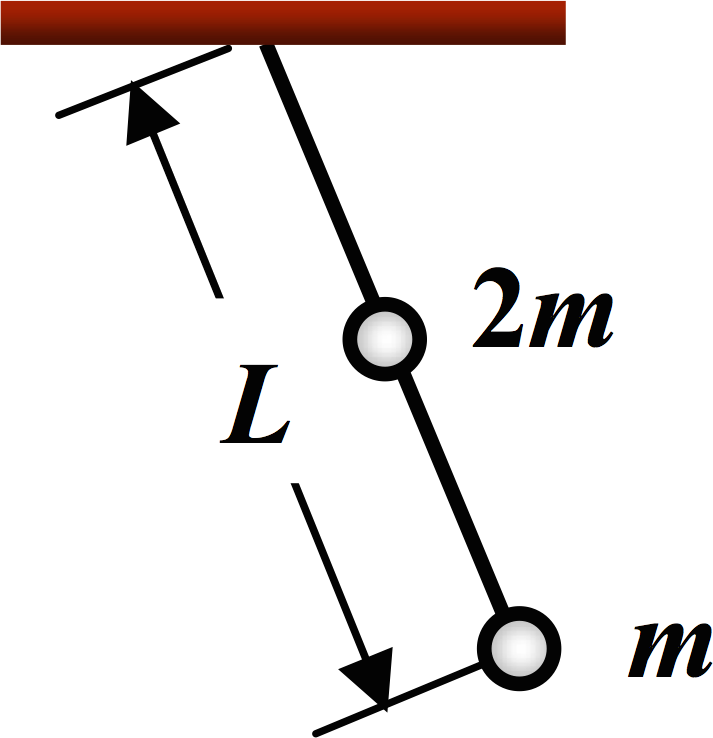
\includegraphics[width=\textwidth]{pendulum.png}}
\end{minipage}
\end{tabular}

\item
A car has an engine which delivers a constant power. It accelerates from rest at time $t=0$, and at $t=t_0$ its acceleration is $a_0$. What is its acceleration at $t=3t_0$? Ignore energy loss due to friction.
\begin{enumerate}
\item $a_0$
\item $2a_0$
\item $3a_0$
\item $a_0/\sqrt{2}$
\item $a_0/\sqrt{3}$
\end{enumerate}

\vfill
\newpage

\item
The elastic collision between two bodies, A and B, can be considered using the following model. A and B are free to move along a common line without friction. When their distance is greater than $d=1$ m, the interacting force is zero; when their distance is less than $d$, a constant repulsive force $F=6$ N is present. The mass of body A is $m_\text{A}=1$ kg and it is initially at rest the mass of body B is $m_\text{B}=3$ kg and it is approaching body A head-on with a speed $v_0=2$ m/s. Find the minimum distance between A and B.

\begin{tabular}{l r}

\begin{minipage}{0.6\textwidth}
\begin{enumerate}
\item 0.25 m
\item 0.50 m
\item 0.75 m
\item 1.00 m
\item 1.25 m
\end{enumerate}
\end{minipage} &
\begin{minipage}{0.3\textwidth}
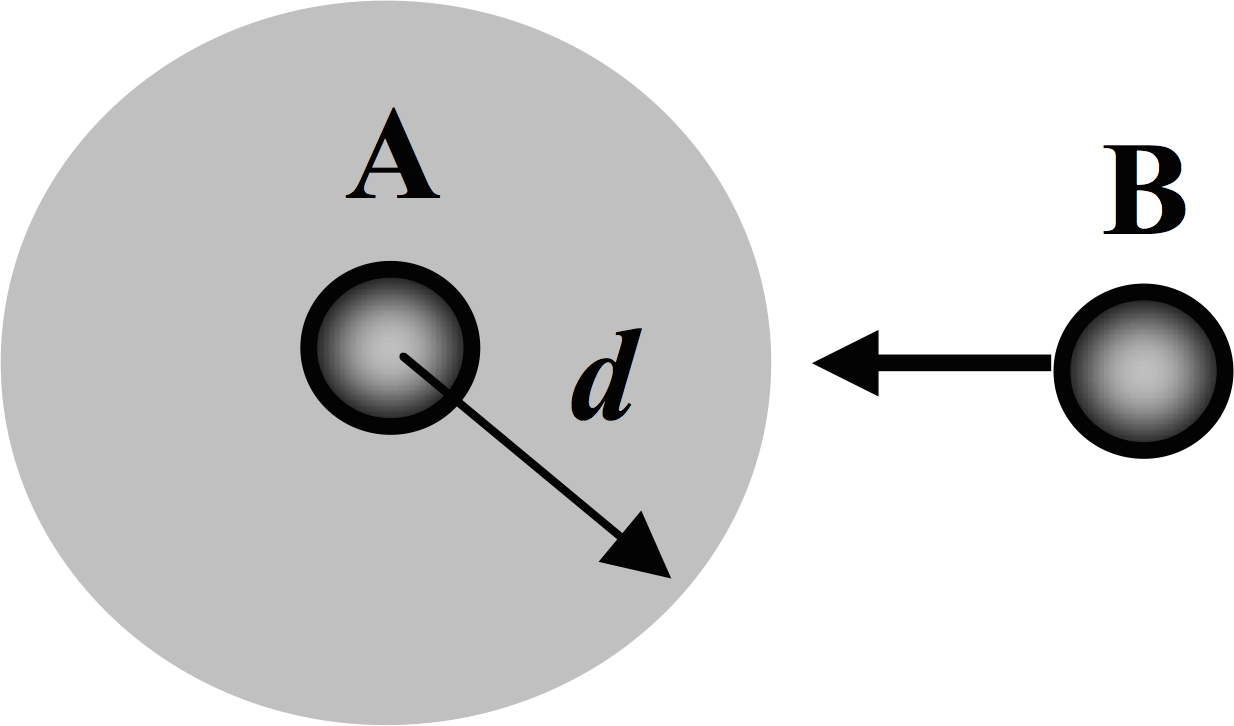
\includegraphics[width=\textwidth]{interaction.png}
\end{minipage}
\end{tabular}

\item
A light glass tube with a sealed lower end and cross-sectional area $A = 2.5$ cm$^2$ contains a column of mercury of mass $m=2$ kg. Between the mercury and the lower end is some trapped gas. The glass tube is sliding down a slope with an inclining angle $\alpha=30\degree$. The coefficient of kinetic friction between the tube and the slope is $\mu=\sqrt{3}/6$. Find the pressure of the trapped gas in terms of the standard atmosphere pressure $P_0=1.0 \times 10^5$ Pa.

\begin{tabular}{l r}

\begin{minipage}{0.6\textwidth}
\begin{enumerate}
\item 1.7
\item 1.2
\item 1.9
\item 2.3
\item 16
\end{enumerate}
\end{minipage} &
\begin{minipage}{0.3\textwidth}
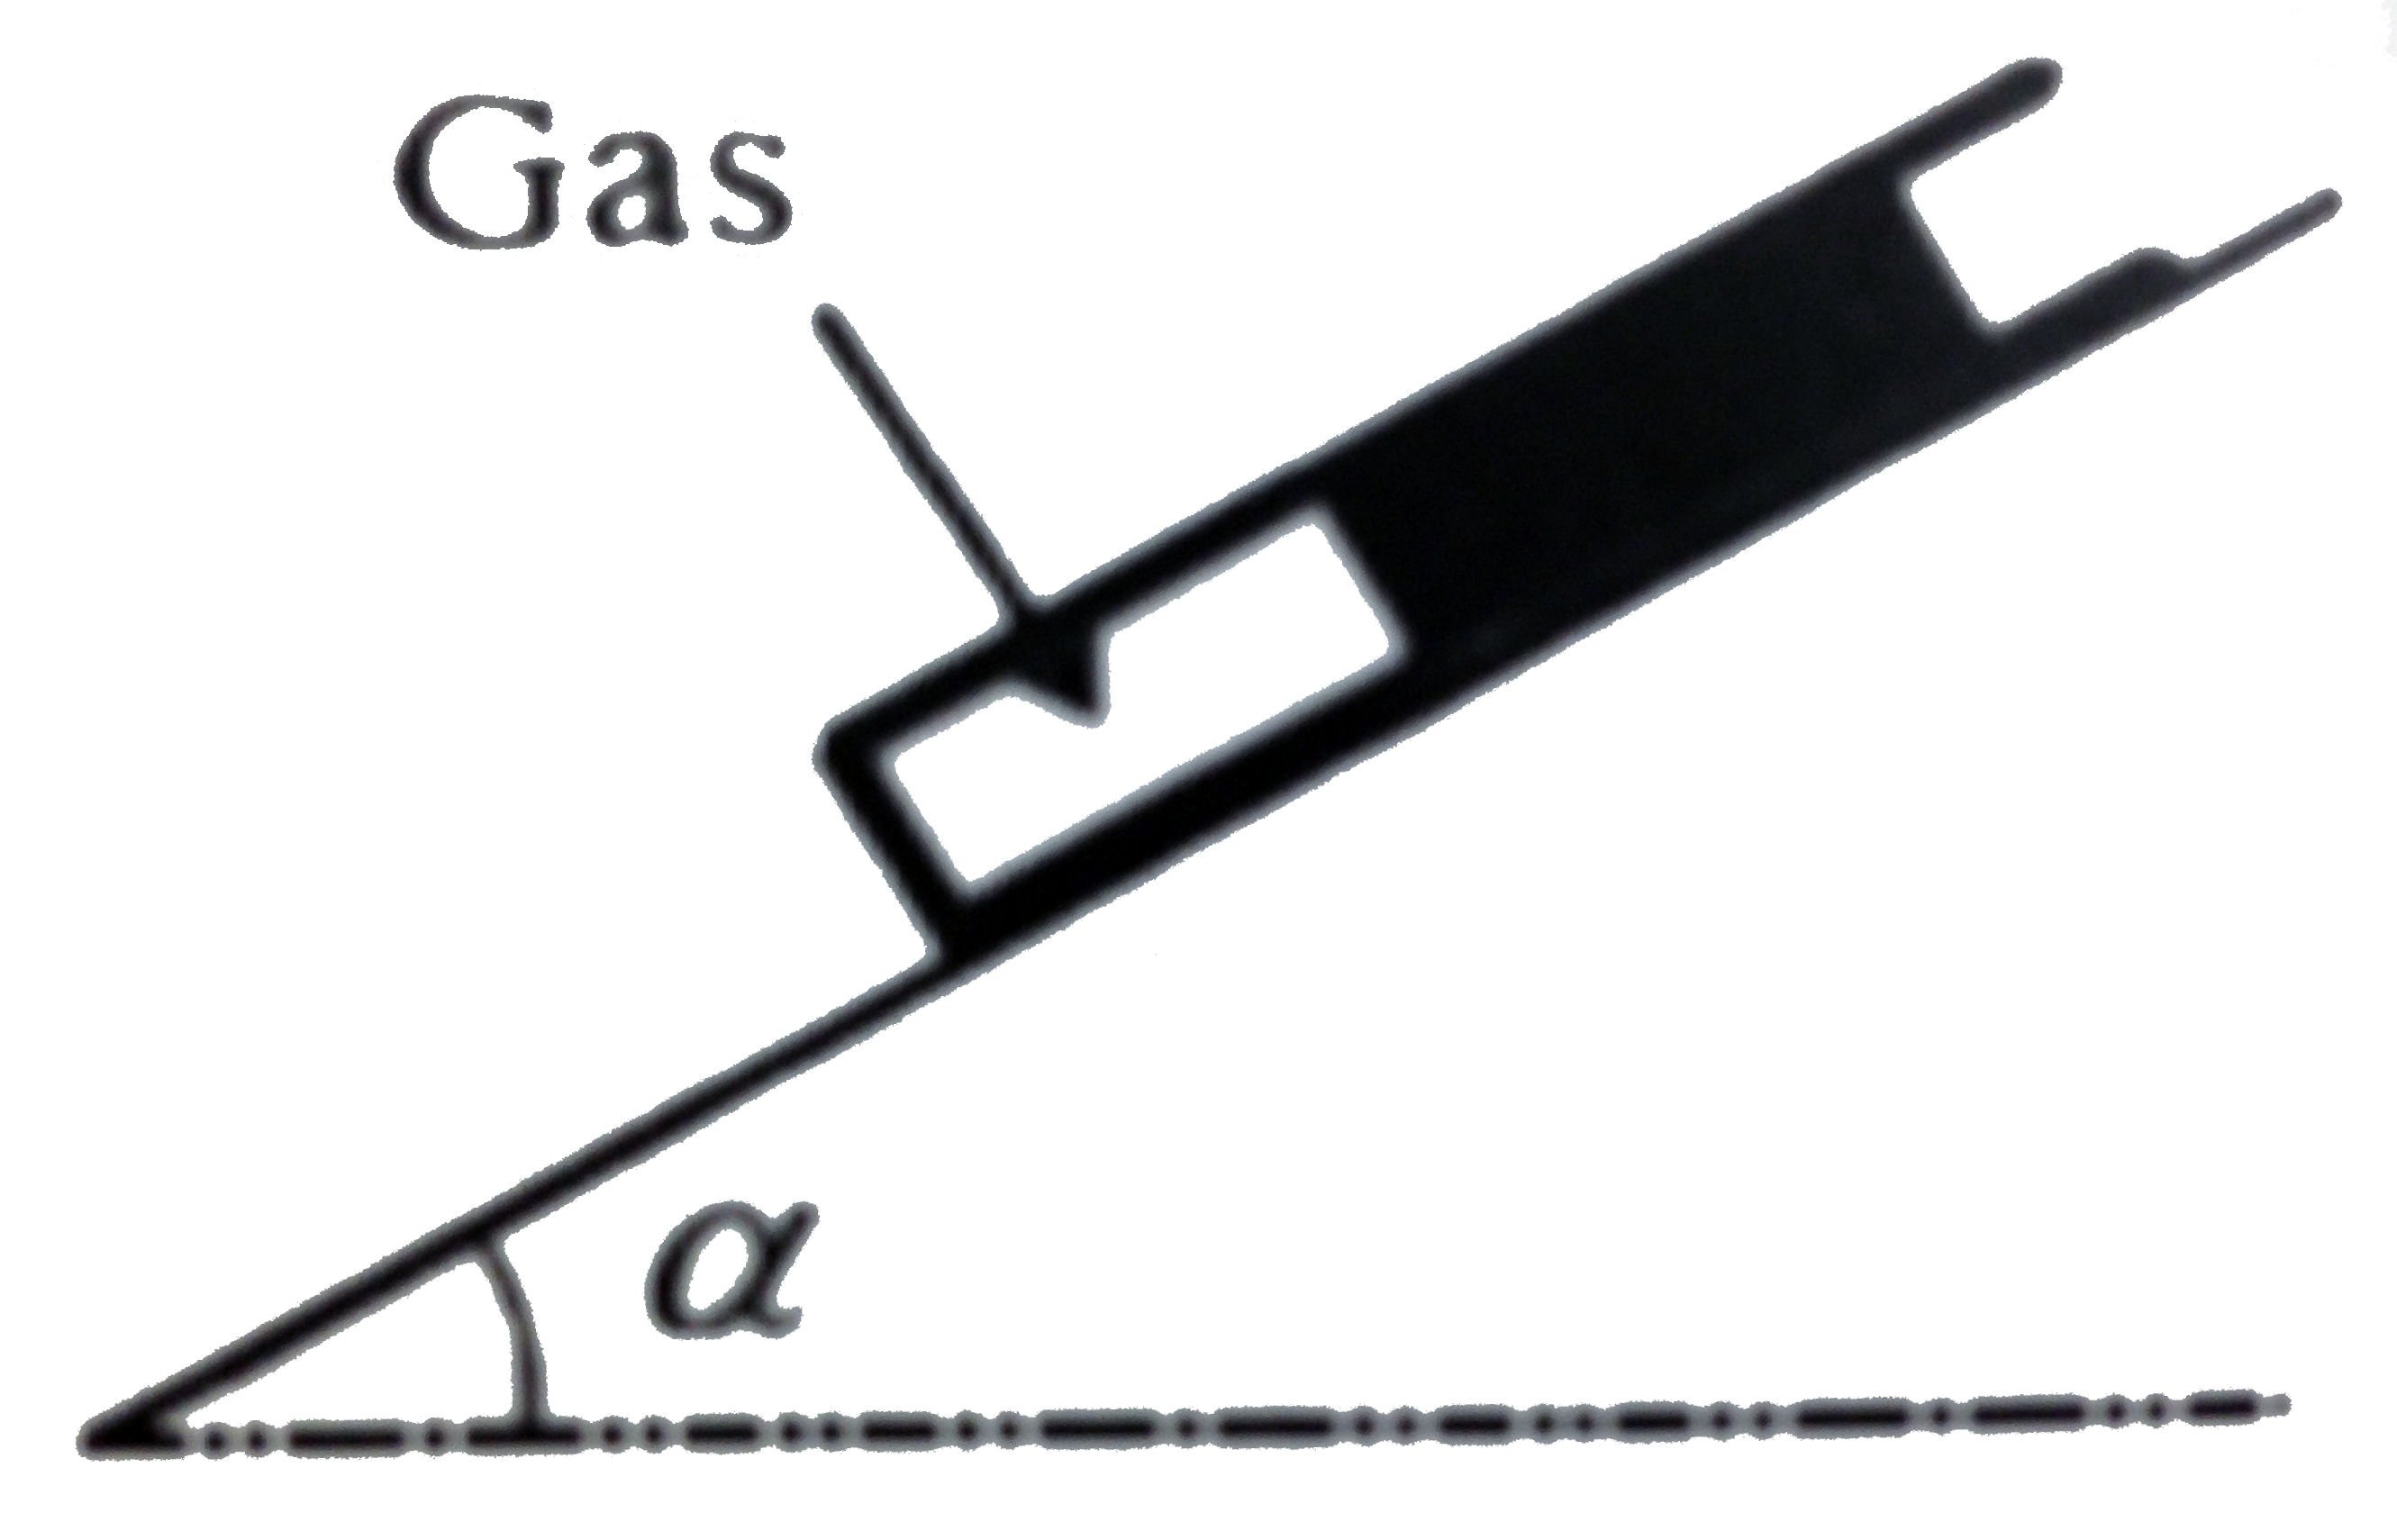
\includegraphics[width=\textwidth]{tube.png}
\end{minipage}
\end{tabular}

\item
A thin circular wooden hoop of mass $m$ and radius $R$ rests on a horizontal frictionless plane. A bullet, also of mass $m$, moving with horizontal velocity $v$, strikes the hoop and becomes embedded in it as shown in the figure. The angular velocity $\omega$ of the hoop after collision is

\begin{tabular}{l r}

\begin{minipage}{0.5\textwidth}
\begin{enumerate}
\item $v/(3R)$
\item $2v/(3R)$
\item $v/R$
\item $v/(6R)$
\item 0
\end{enumerate}
\end{minipage} &
\begin{minipage}{0.4\textwidth}
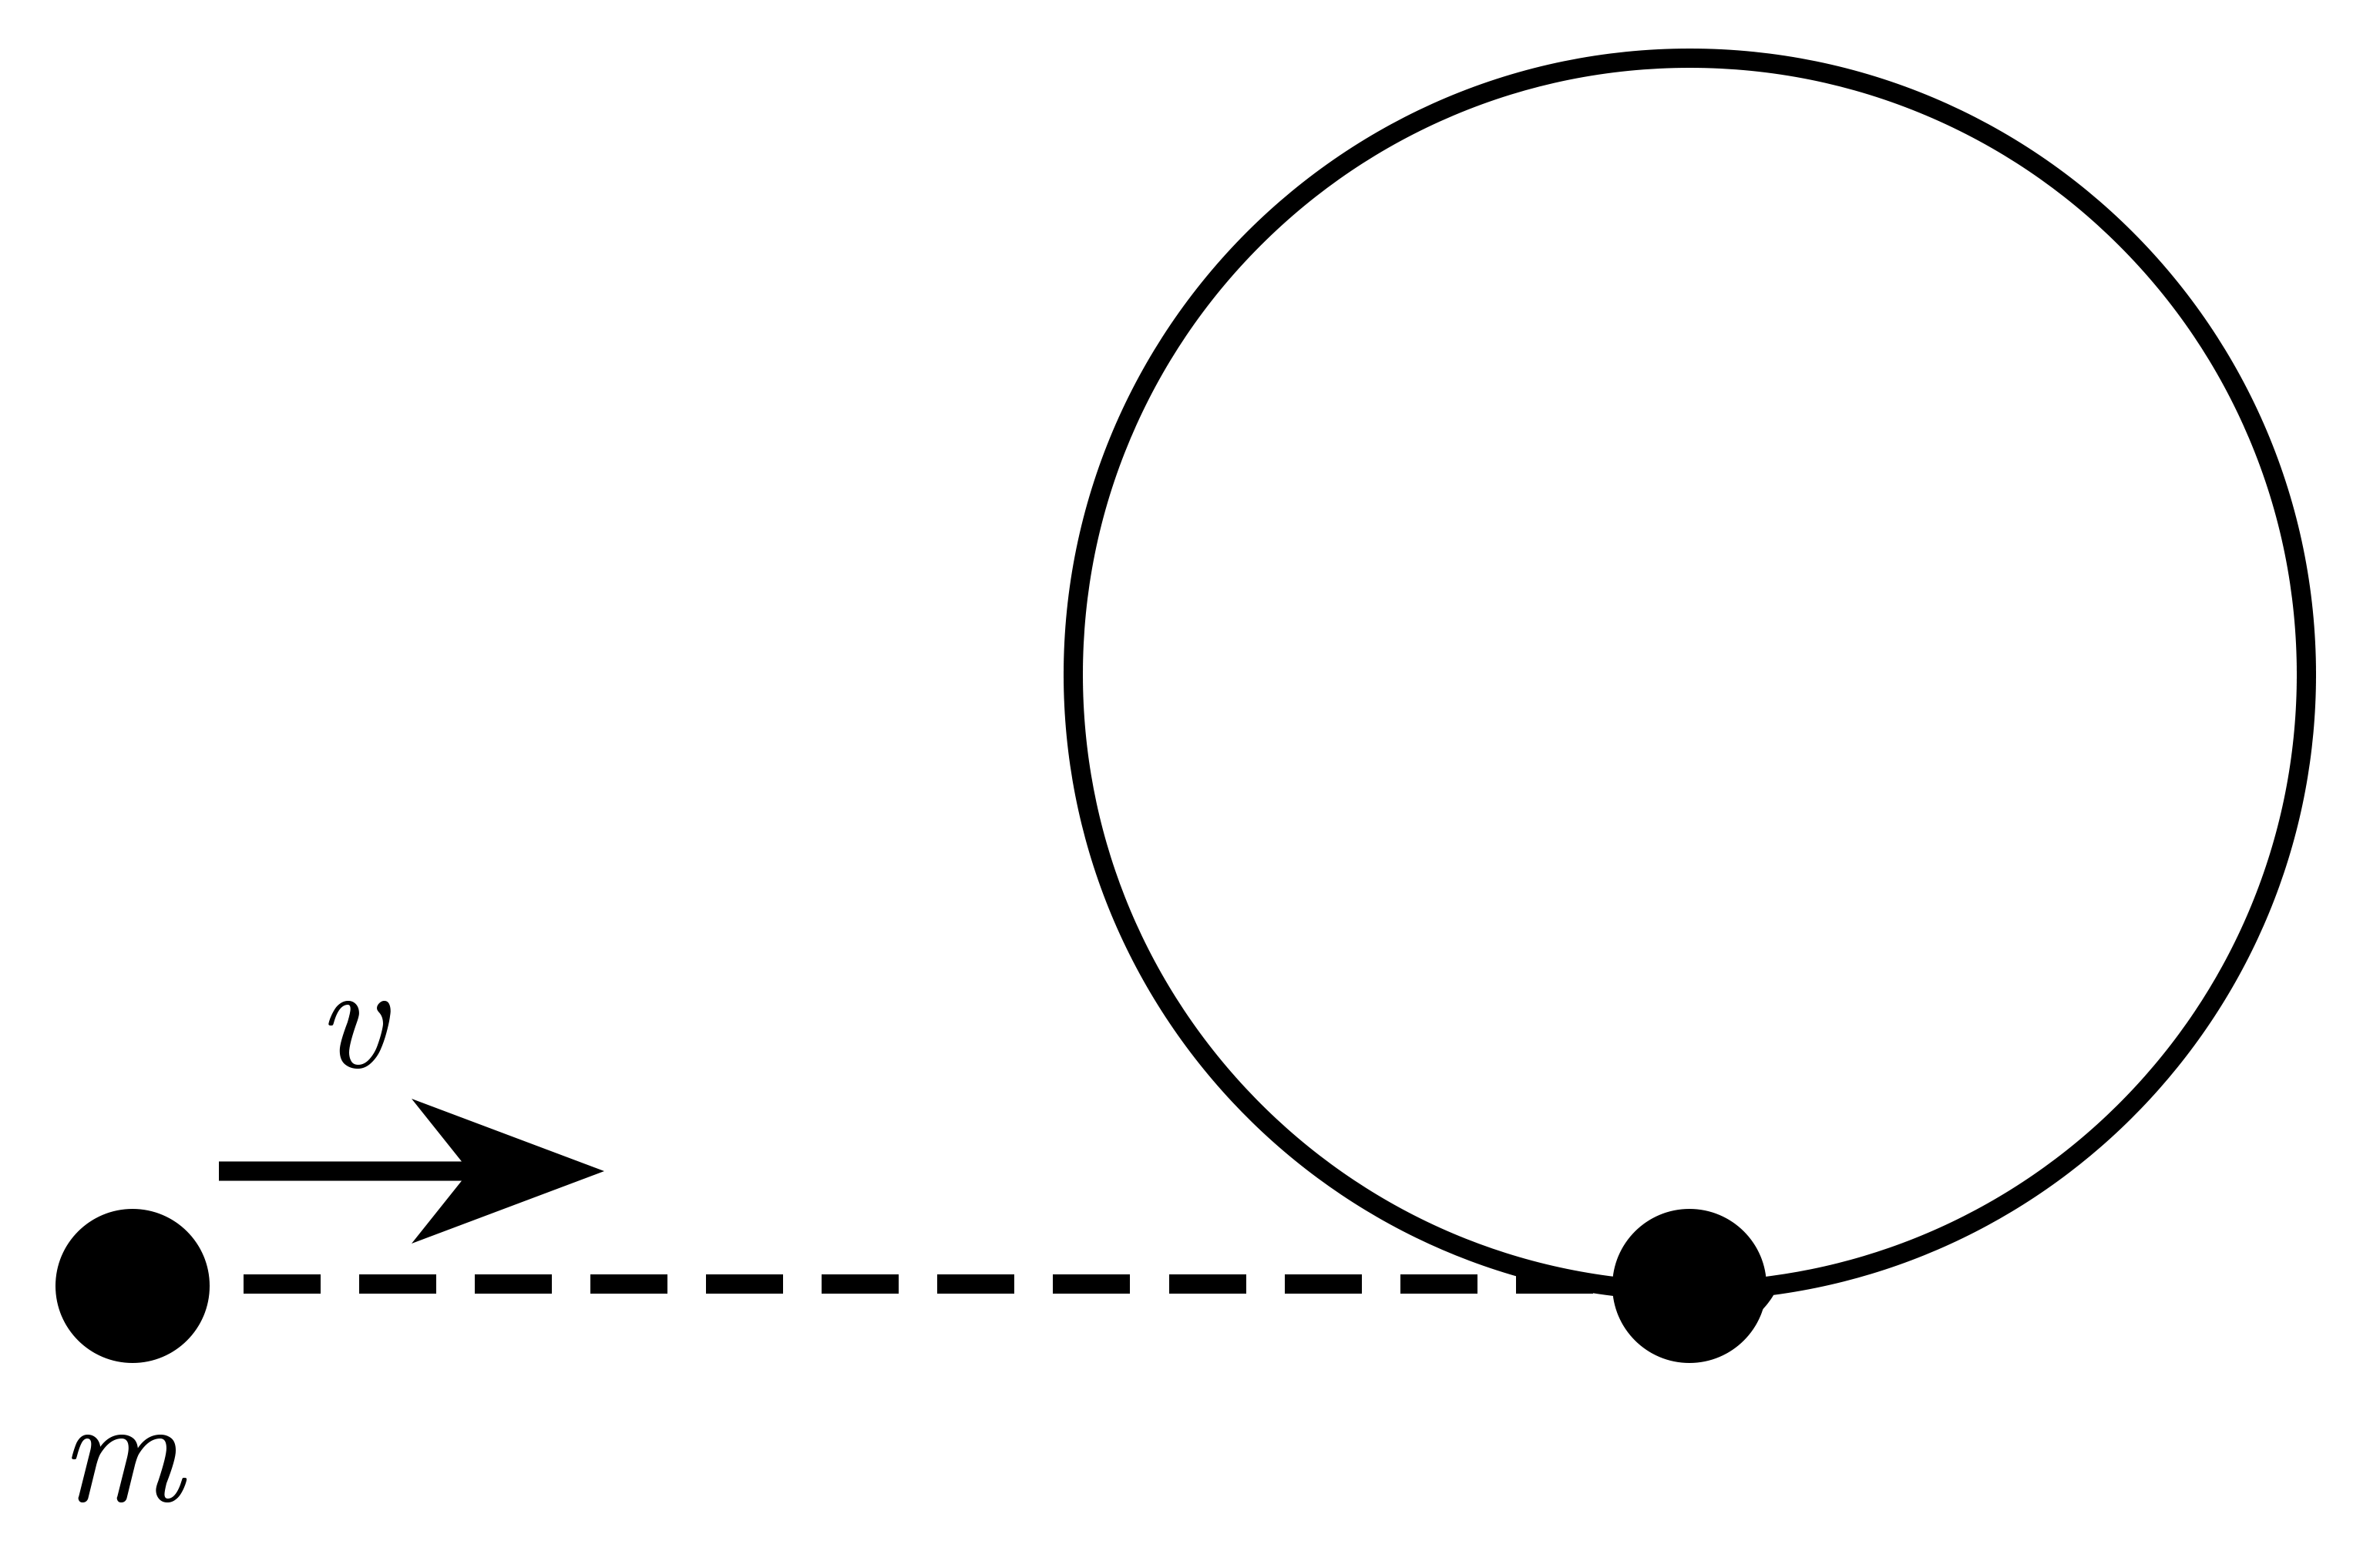
\includegraphics[width=\textwidth]{hoop.png}
\end{minipage}
\end{tabular}

\end{enumerate}
\end{document}
